In this subsection are presented the results of the parallel version of Tarjan's algorithm with CUDA with the use of the texture memory.
Each graph is tested with all the compiler optimization (O0, O1, O2, O3) and with $\frac{n}{4}$, $\frac{n}{2}$, $\frac{3*n}{4}$, $n$ CUDA threads, where $n$ is the number of vertices of the graph tested.  
In the next pages for each graph, set the optimization, there are a table and a graph of the speedup.
In the table there are:
\begin{itemize}
    \item \textbf{Version}: is the version of the program. It can be "Serial" if it's the sequential with preprocessing version of the program, or it can be "Parallel" if it's the parallel version with CUDA.
    \item \textbf{Threads}: is the number of thread CUDA. For the "Serial" version, the value of this field is 1, because it's the sequential with preprocessing version of the program executed on only one processor of the CPU.
    \item \textbf{vertices}: is the number of vertices of the graph after the preprocessing.
    \item \textbf{init}: is the time spent to initialize the program, in particular it's the time spent to create and initialize the data structures, and to read the graph from a file.
    \item \textbf{preprocess}: is the time spent to do the preprocessing of the graph.
    \item \textbf{conversion}: is the time spent to convert the graph into a graph adapted for CUDA.
    \item \textbf{finalize}: is the time spent to deallocate the necessary data structures.
    \item \textbf{tarjan}: the time spent to execute Tarjan's algorithm.
    \item \textbf{user}: is the total number of CPU-seconds that the process used directly (in user mode), in seconds.
    \item \textbf{system}: is the total number of CPU-seconds used by the system on behalf of the process (in kernel mode), in seconds.
    \item \textbf{pCPU}: is the percentage of the CPU that this process got. This is just user + system times divided by the total running time.
    \item \textbf{elapsed}: is the elapsed real (wall clock) time used by the process, in seconds.
    \item \textbf{Speedup}: the speedup of the program.
    \item \textbf{Efficiency}: the efficiency of the program.
\end{itemize}
All values except those in the \verb|Version|, \verb|Threads|, \verb|Speedup|, and \verb|Efficiency| columns are means. These means were calculated from the files of the measurements taken.
\verb|Speedup|, and \verb|Efficiency| are calculated with the formulas in Cap.\ref{ch:1} using the results of these means.
For the sequential algorithm, the \verb|finalize| and \verb|conversion| fields were not measured. 

%Fully connected graph
\clearpage
\subsection{Fully connected graph}
\subsubsection{Optimization 0}
\begin{center}
    \resizebox{0.8\textwidth}{!}{\subfile{../tables/psize-graph_type-fully-connected-12500-O0-table}}
    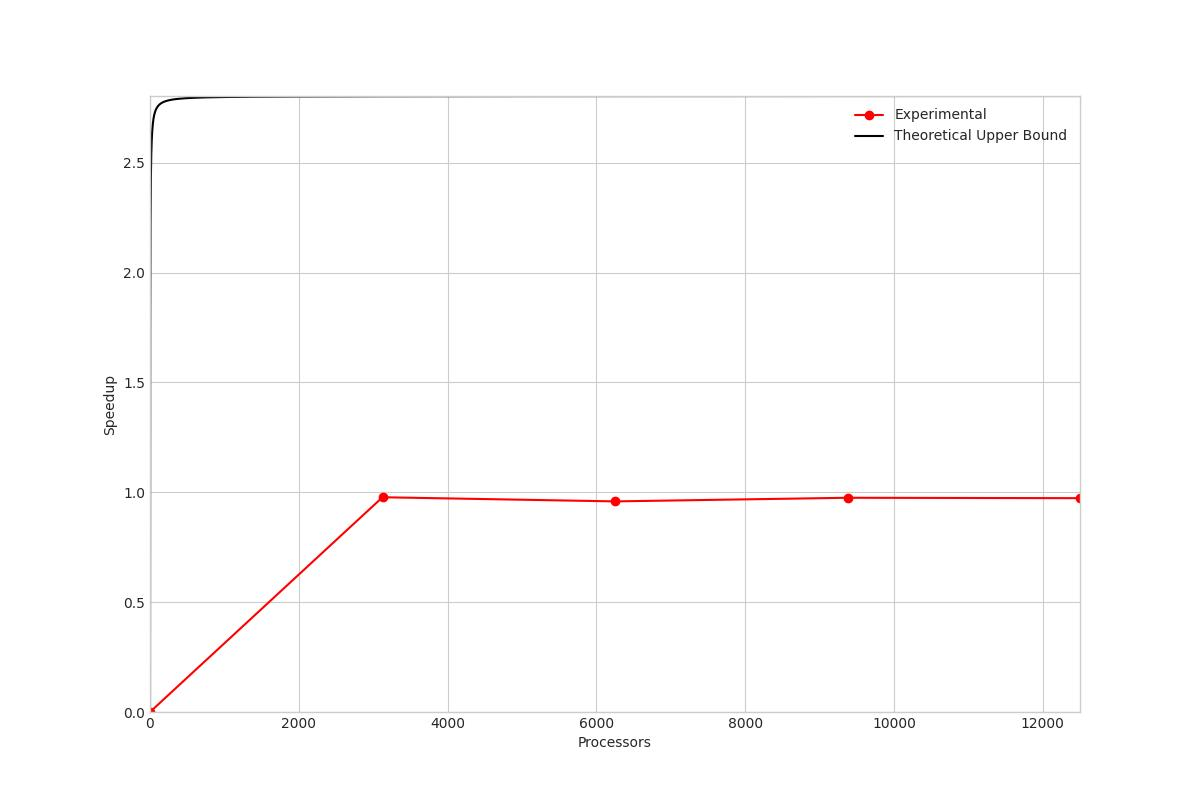
\includegraphics[width=0.74\textwidth]{../img/speedup-graph_type-fully-connected-12500-O0}
\end{center}

\subsubsection{Optimization 1}
\begin{center}
    \resizebox{0.8\textwidth}{!}{\subfile{../tables/psize-graph_type-fully-connected-12500-O1-table}}
    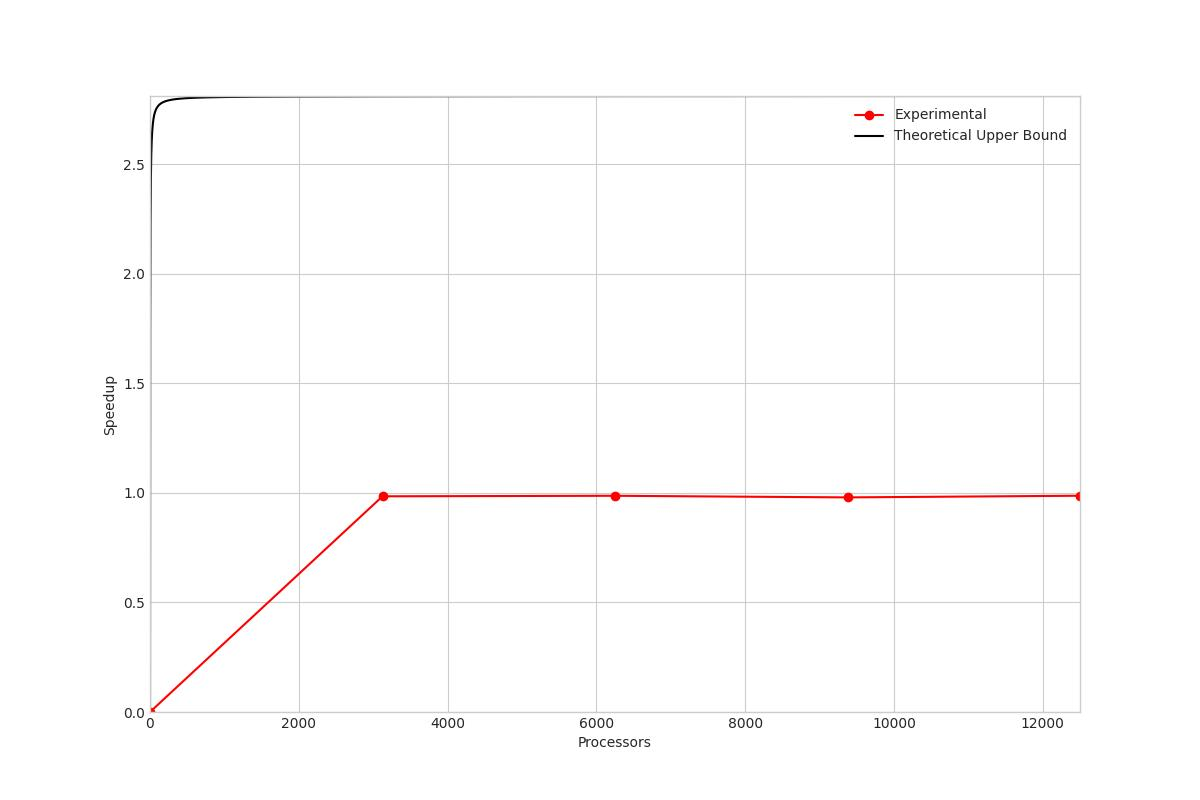
\includegraphics[width=0.74\textwidth]{../img/speedup-graph_type-fully-connected-12500-O1}
\end{center}

\clearpage
\subsubsection{Optimization 2}
\begin{center}
    \resizebox{0.8\textwidth}{!}{\subfile{../tables/psize-graph_type-fully-connected-12500-O2-table}}
    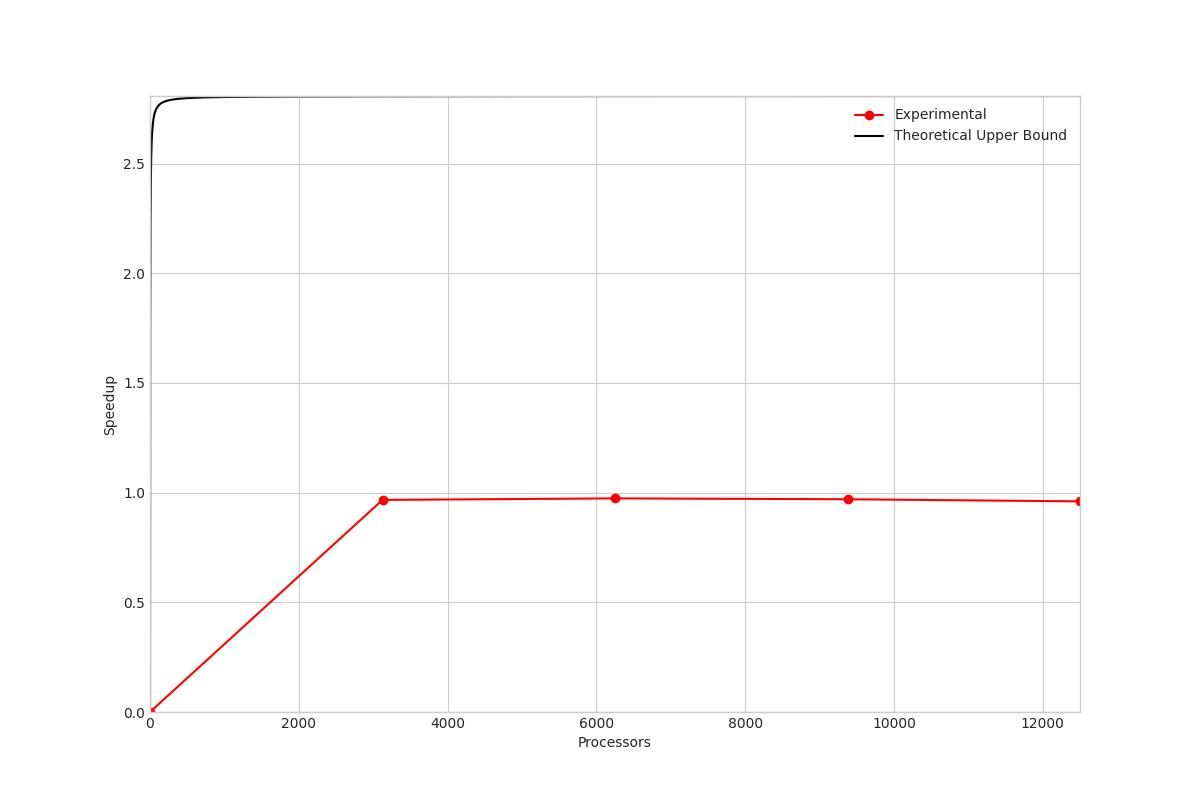
\includegraphics[width=0.78\textwidth]{../img/speedup-graph_type-fully-connected-12500-O2}
\end{center}

\subsubsection{Optimization 3}
\begin{center}
    \resizebox{0.8\textwidth}{!}{\subfile{../tables/psize-graph_type-fully-connected-12500-O3-table}}
    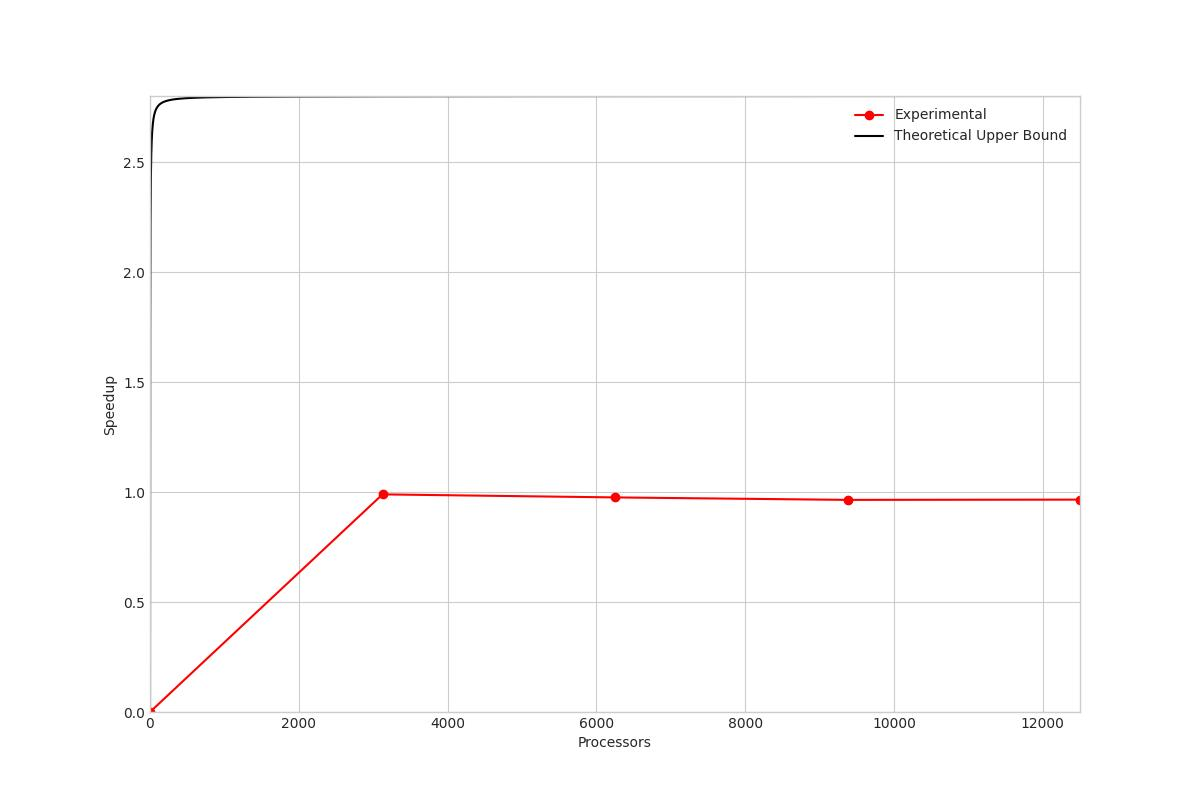
\includegraphics[width=0.78\textwidth]{../img/speedup-graph_type-fully-connected-12500-O3}
\end{center}

%Fully disconnected graph
\clearpage
\subsection{Fully disconnected graph}
\subsubsection{Optimization 0}
\begin{center}
    \resizebox{0.8\textwidth}{!}{\subfile{../tables/psize-graph_type-fully-disconnected-1000000-O0-table}}
    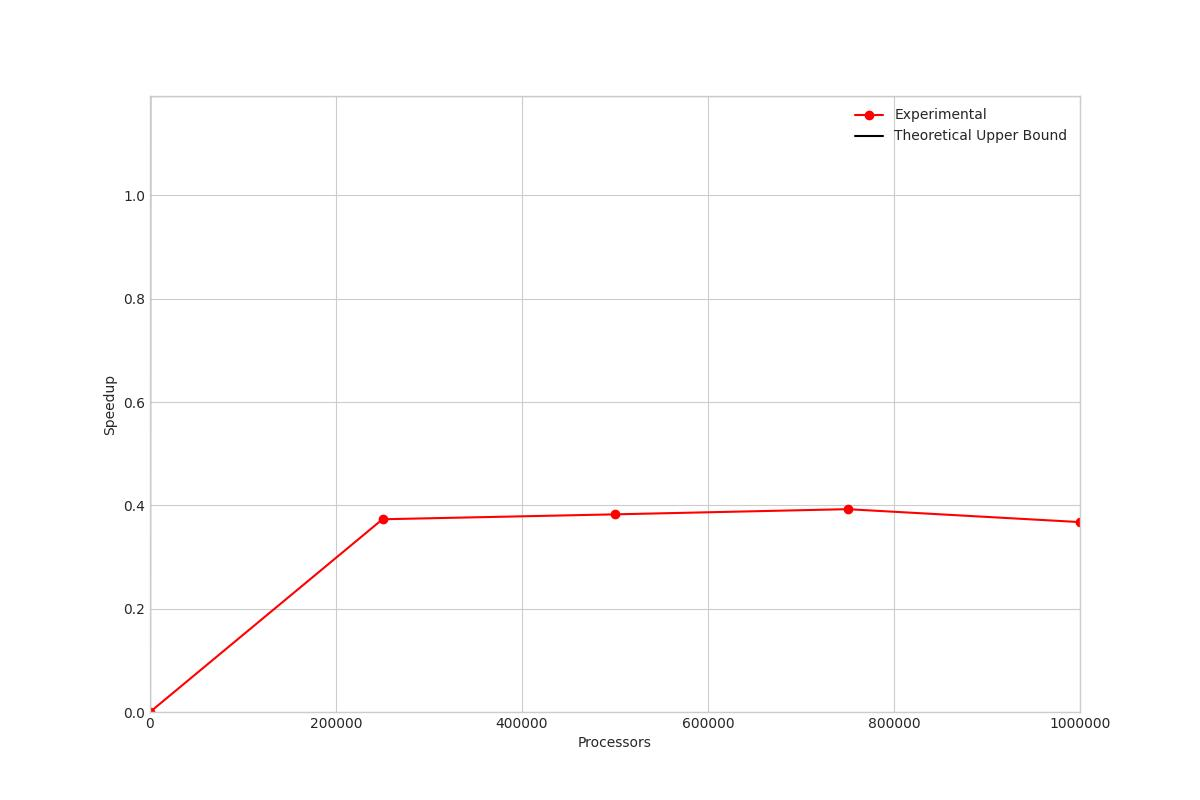
\includegraphics[width=0.73\textwidth]{../img/speedup-graph_type-fully-disconnected-1000000-O0}
\end{center}

\subsubsection{Optimization 1}
\begin{center}
    \resizebox{0.8\textwidth}{!}{\subfile{../tables/psize-graph_type-fully-disconnected-1000000-O1-table}}
    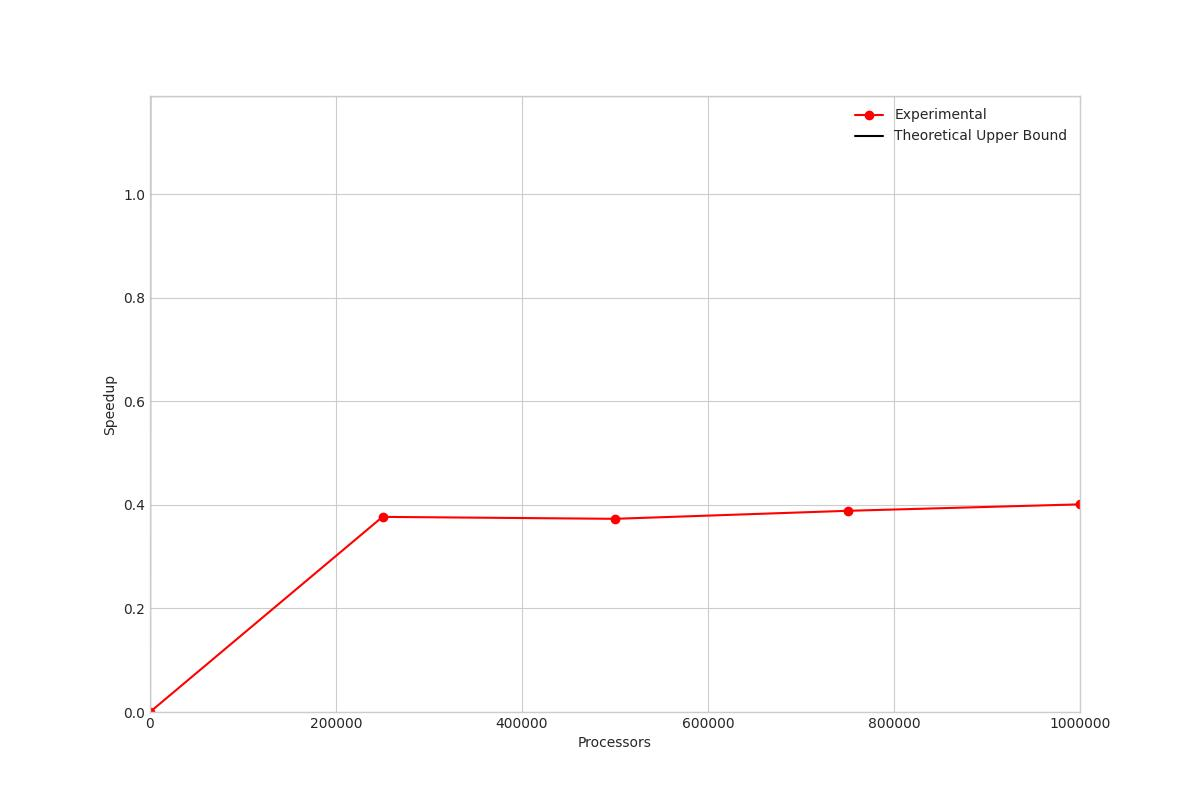
\includegraphics[width=0.74\textwidth]{../img/speedup-graph_type-fully-disconnected-1000000-O1}
\end{center}

\clearpage
\subsubsection{Optimization 2}
\begin{center}
    \resizebox{0.8\textwidth}{!}{\subfile{../tables/psize-graph_type-fully-disconnected-1000000-O2-table}}
    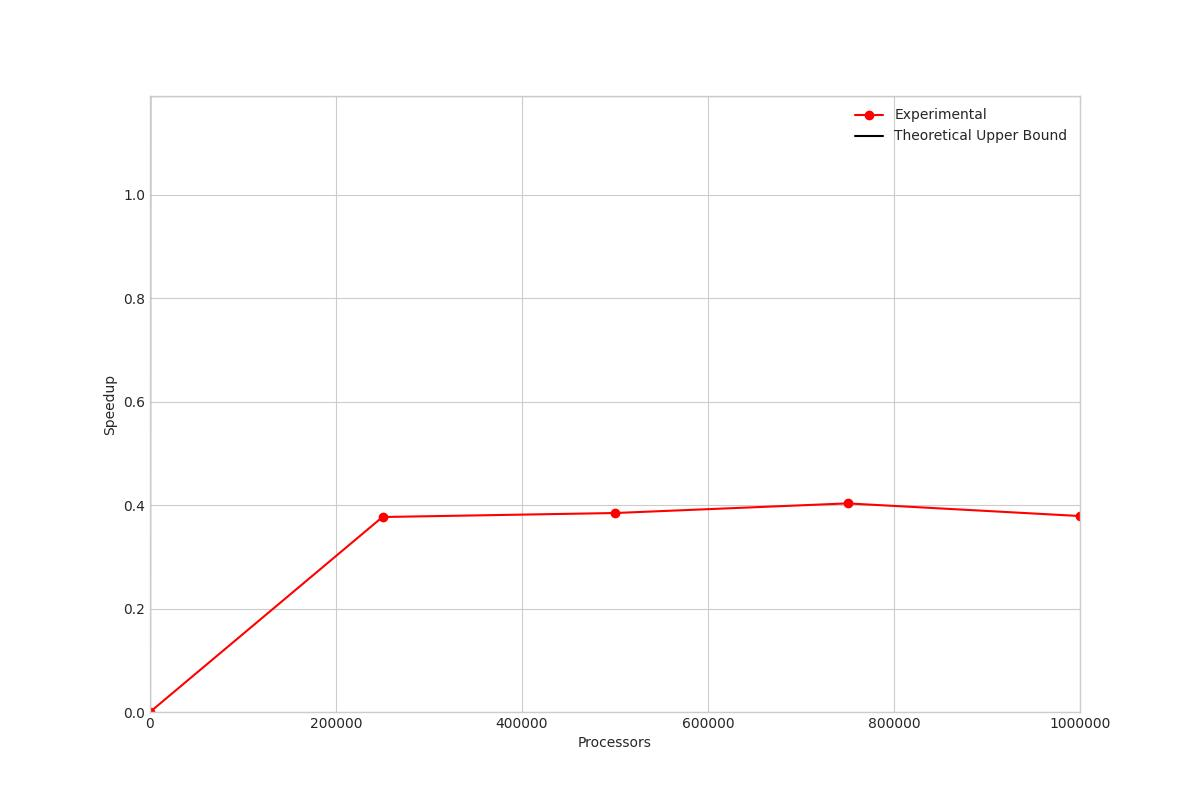
\includegraphics[width=0.77\textwidth]{../img/speedup-graph_type-fully-disconnected-1000000-O2}
\end{center}

\subsubsection{Optimization 3}
\begin{center}
    \resizebox{0.8\textwidth}{!}{\subfile{../tables/psize-graph_type-fully-disconnected-1000000-O3-table}}
    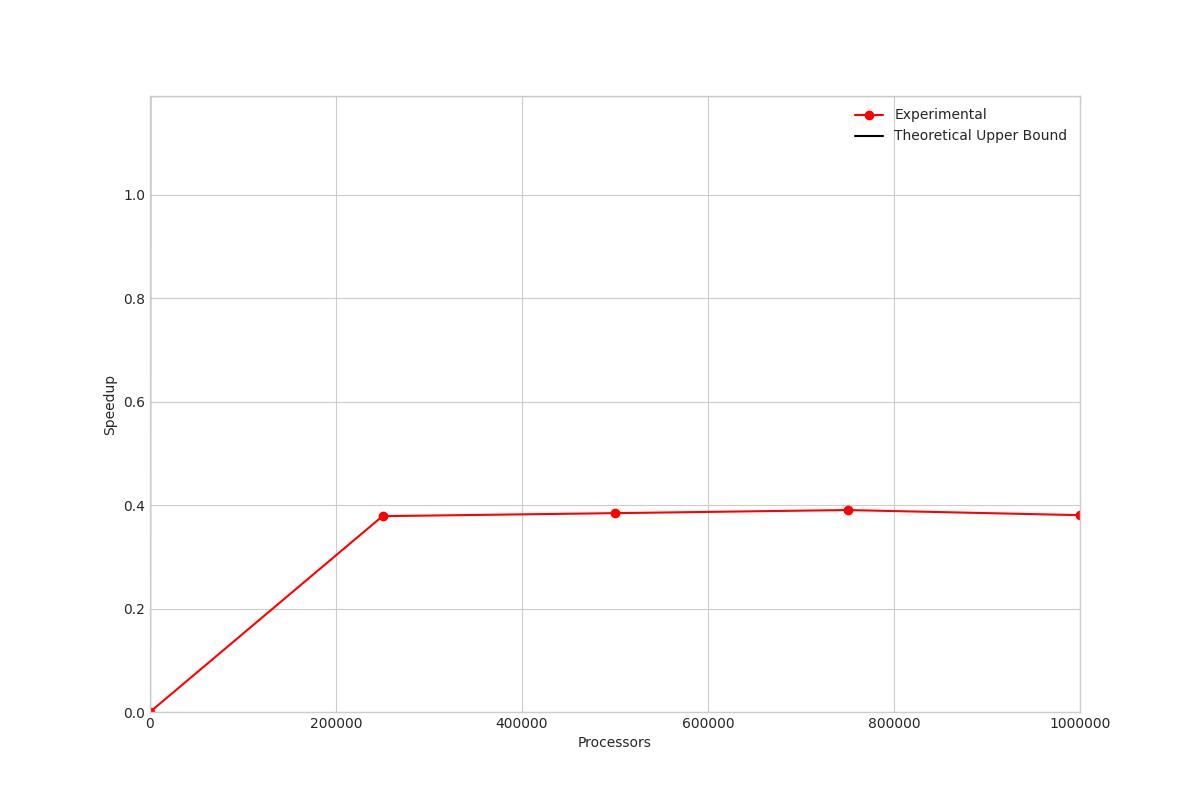
\includegraphics[width=0.77\textwidth]{../img/speedup-graph_type-fully-disconnected-1000000-O3}
\end{center}

%Random-150000 graph
\clearpage
\subsection{Random-150000 graph}
\subsubsection{Optimization 0}
\begin{center}
    \resizebox{0.8\textwidth}{!}{\subfile{../tables/psize-graph_type-random-150000-O0-table}}
    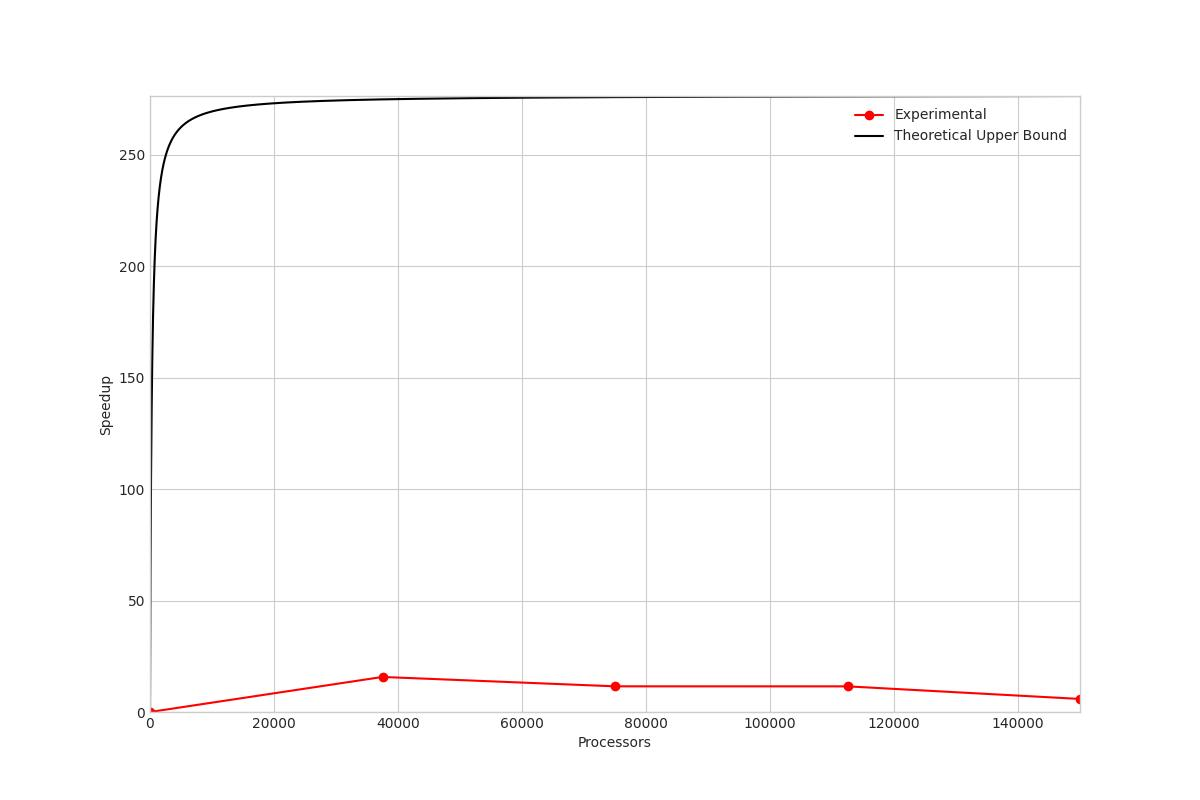
\includegraphics[width=0.74\textwidth]{../img/speedup-graph_type-random-150000-O0}
\end{center}


\subsubsection{Optimization 1}
\begin{center}
    \resizebox{0.8\textwidth}{!}{\subfile{../tables/psize-graph_type-random-150000-O1-table}}
    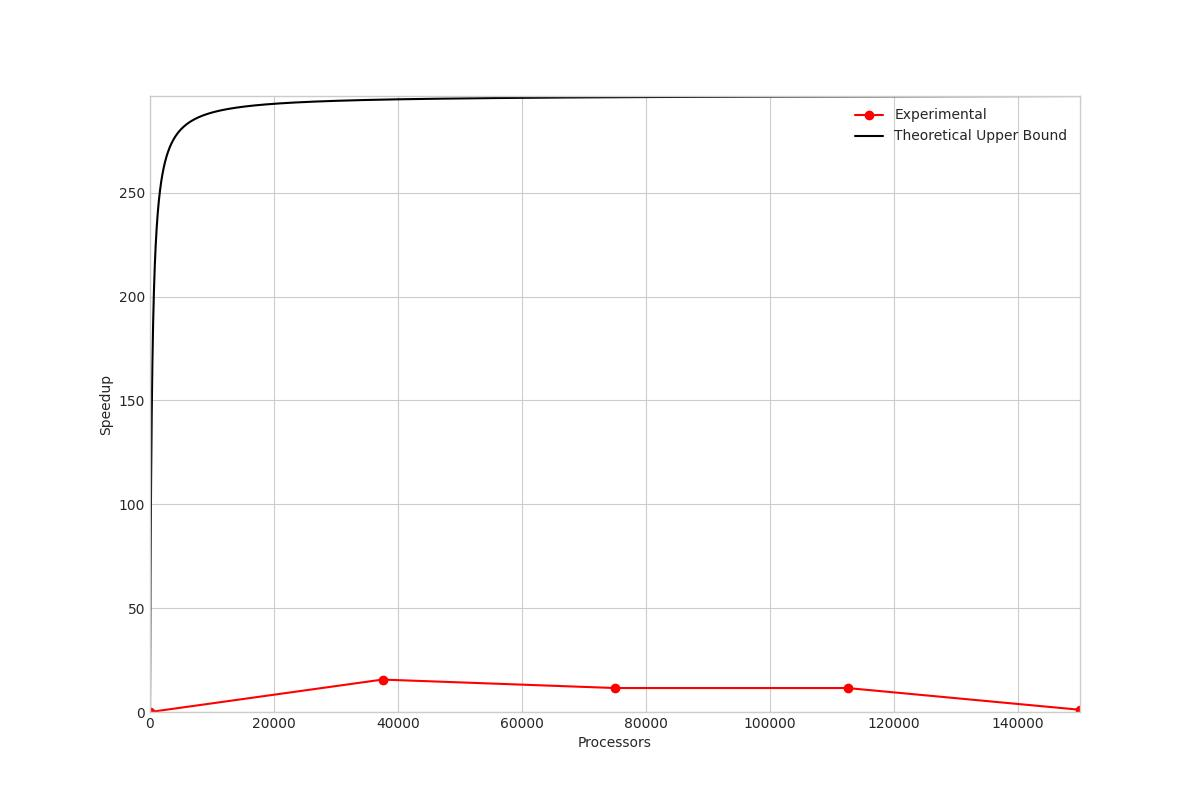
\includegraphics[width=0.74\textwidth]{../img/speedup-graph_type-random-150000-O1}
\end{center}

\clearpage
\subsubsection{Optimization 2}
\begin{center}
    \resizebox{0.8\textwidth}{!}{\subfile{../tables/psize-graph_type-random-150000-O2-table}}
    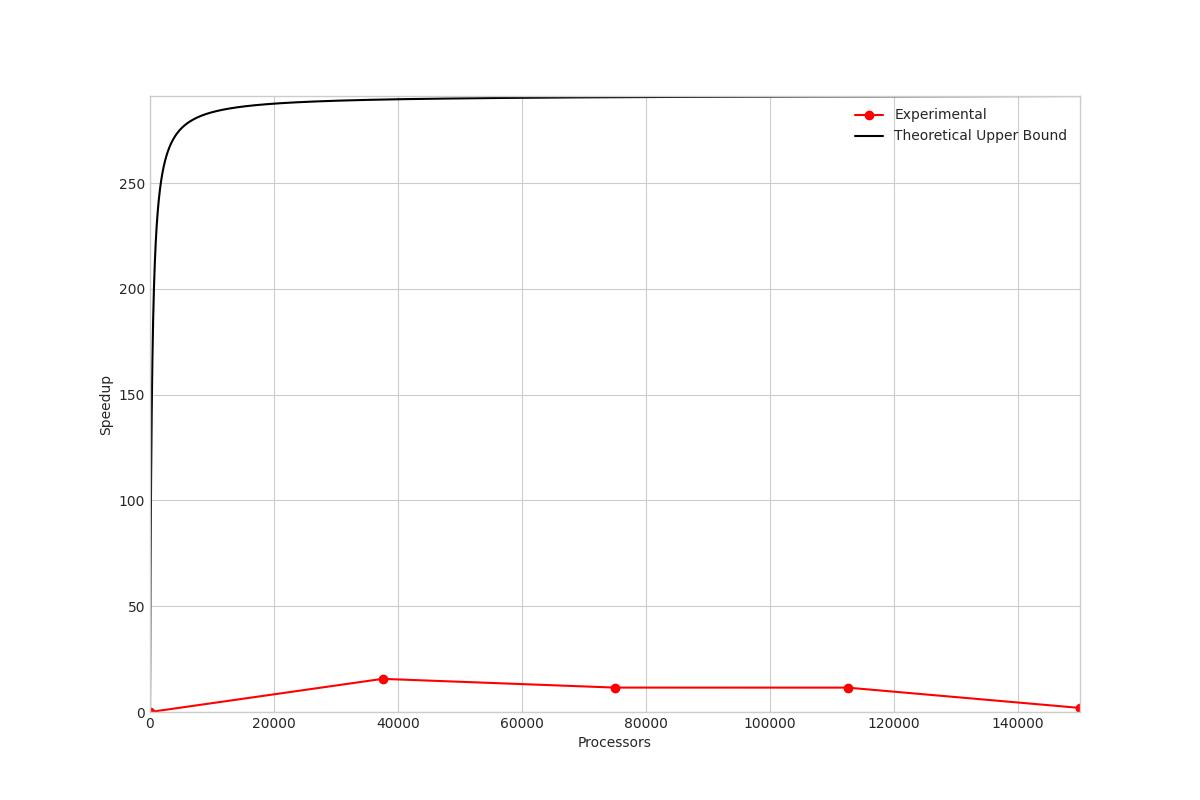
\includegraphics[width=0.78\textwidth]{../img/speedup-graph_type-random-150000-O2}
\end{center}

\subsubsection{Optimization 3}
\begin{center}
    \resizebox{0.8\textwidth}{!}{\subfile{../tables/psize-graph_type-random-150000-O3-table}}
    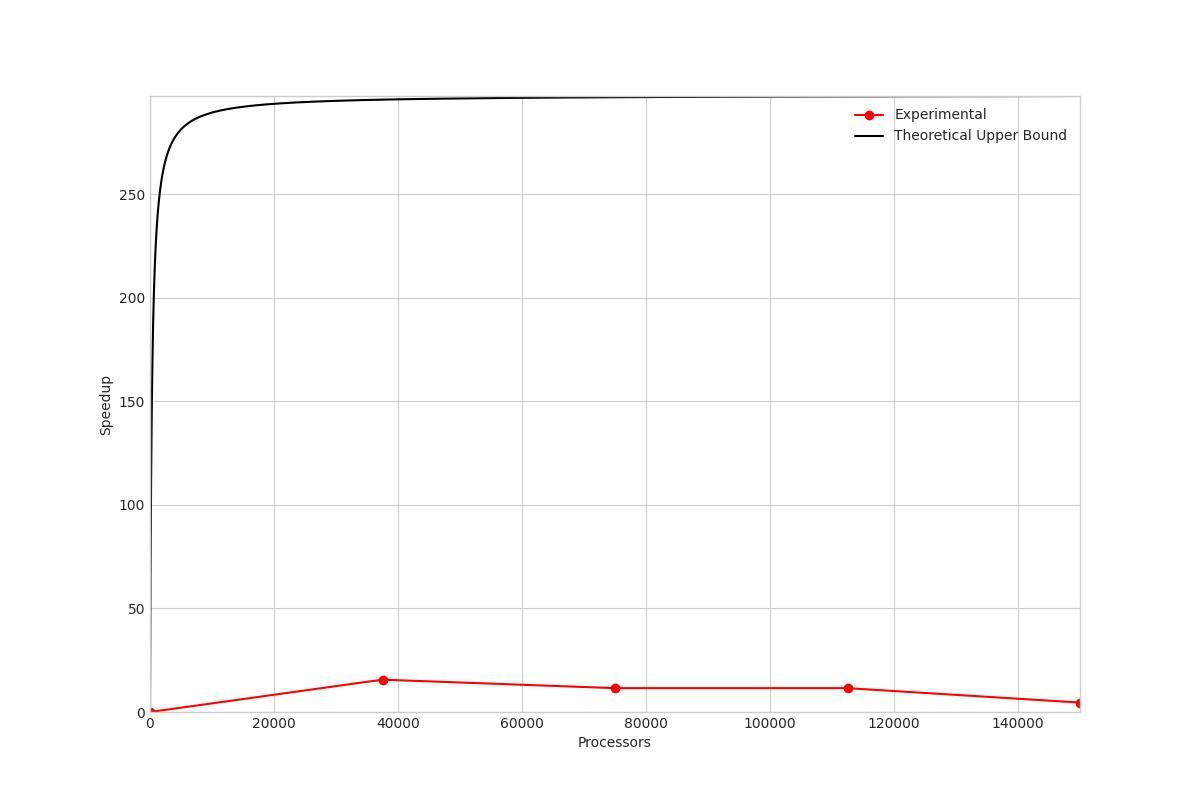
\includegraphics[width=0.78\textwidth]{../img/speedup-graph_type-random-150000-O3}
\end{center}

%Random-250000 graph
\clearpage
\subsection{Random-250000 graph}
\subsubsection{Optimization 0}
\begin{center}
    \resizebox{0.8\textwidth}{!}{\subfile{../tables/psize-graph_type-random-250000-O0-table}}
    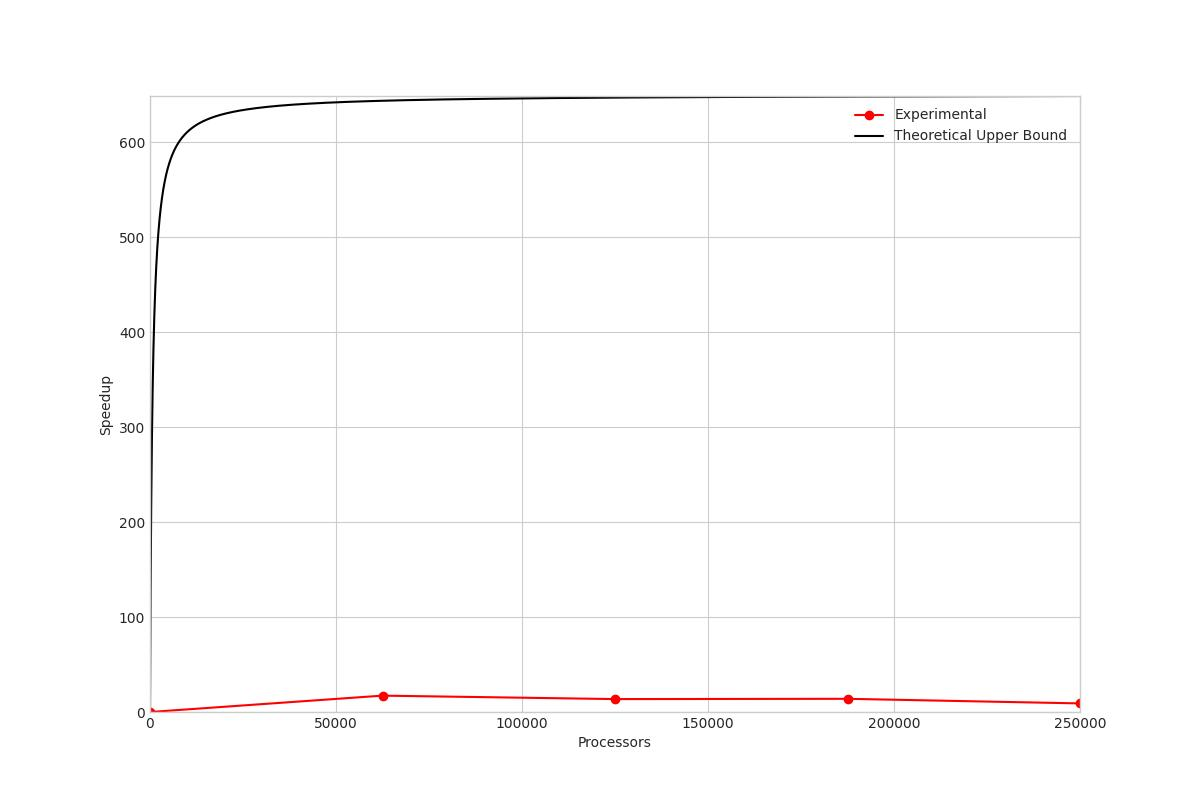
\includegraphics[width=0.74\textwidth]{../img/speedup-graph_type-random-250000-O0}
\end{center}

\subsubsection{Optimization 1}
\begin{center}
    \resizebox{0.8\textwidth}{!}{\subfile{../tables/psize-graph_type-random-250000-O1-table}}
    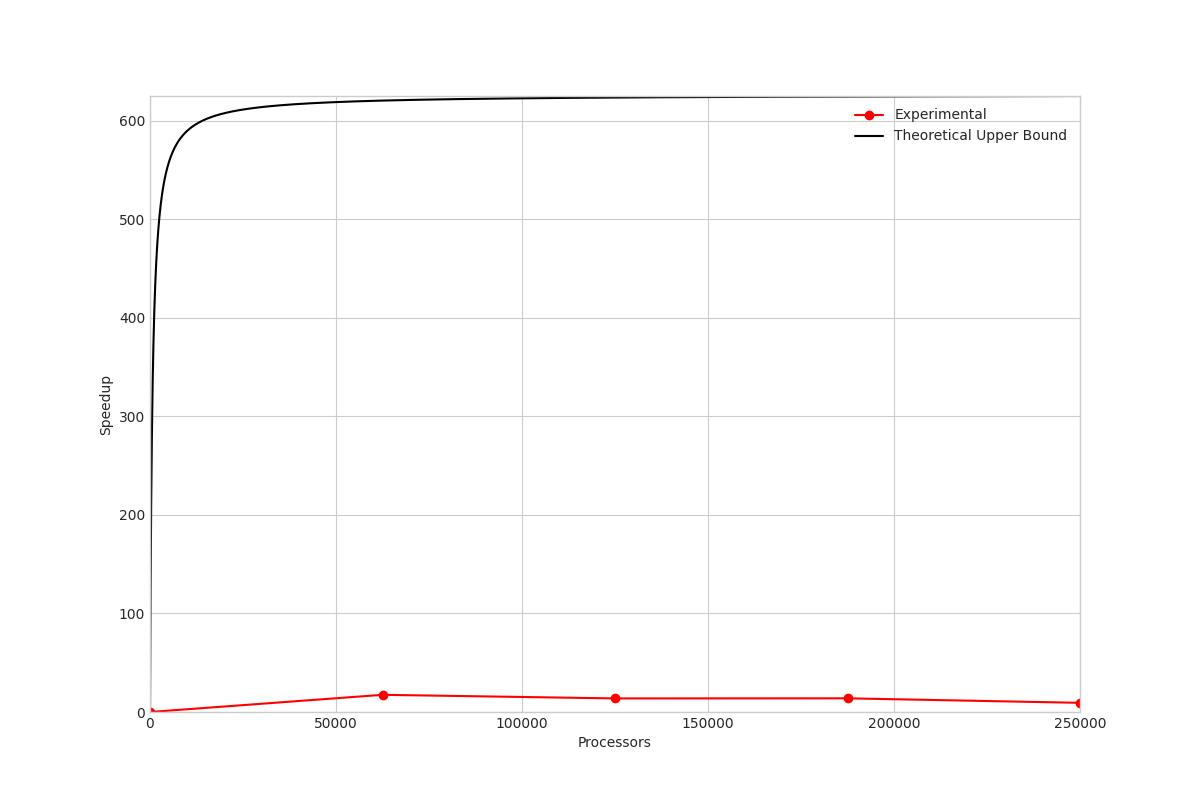
\includegraphics[width=0.74\textwidth]{../img/speedup-graph_type-random-250000-O1}
\end{center}

\clearpage
\subsubsection{Optimization 2}
\begin{center}
    \resizebox{0.8\textwidth}{!}{\subfile{../tables/psize-graph_type-random-250000-O2-table}}
    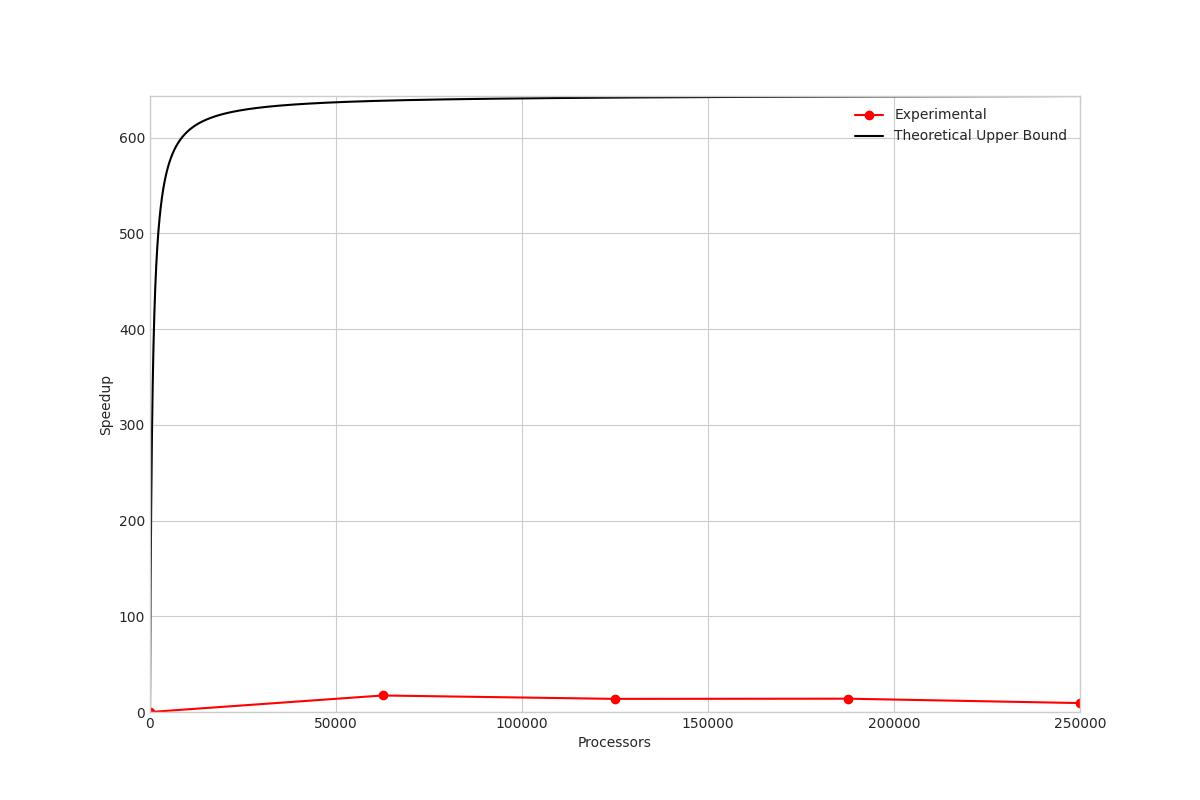
\includegraphics[width=0.78\textwidth]{../img/speedup-graph_type-random-250000-O2}
\end{center}

\subsubsection{Optimization 3}
\begin{center}
    \resizebox{0.8\textwidth}{!}{\subfile{../tables/psize-graph_type-random-250000-O3-table}}
    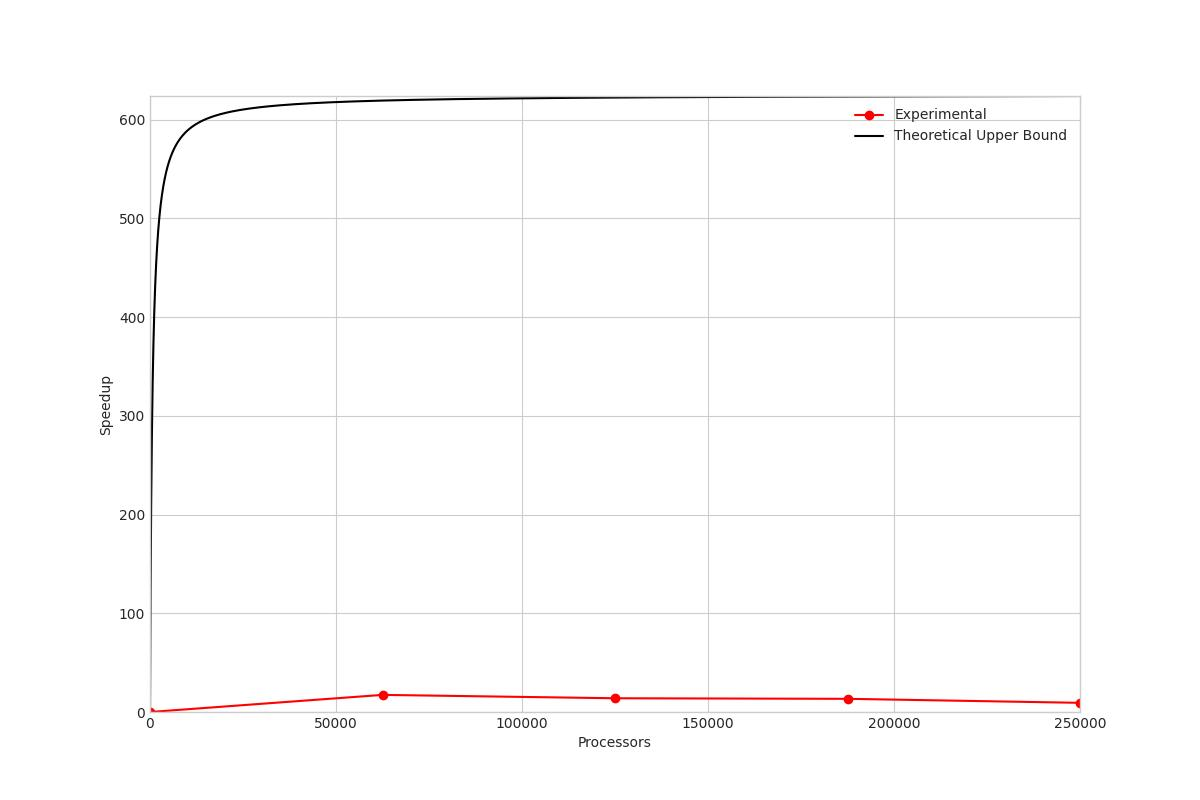
\includegraphics[width=0.78\textwidth]{../img/speedup-graph_type-random-250000-O3}
\end{center}

%Random-500000 graph
\clearpage
\subsection{Random-500000 graph}
\subsubsection{Optimization 0}
\begin{center}
    \resizebox{0.8\textwidth}{!}{\subfile{../tables/psize-graph_type-random-500000-O0-table}}
    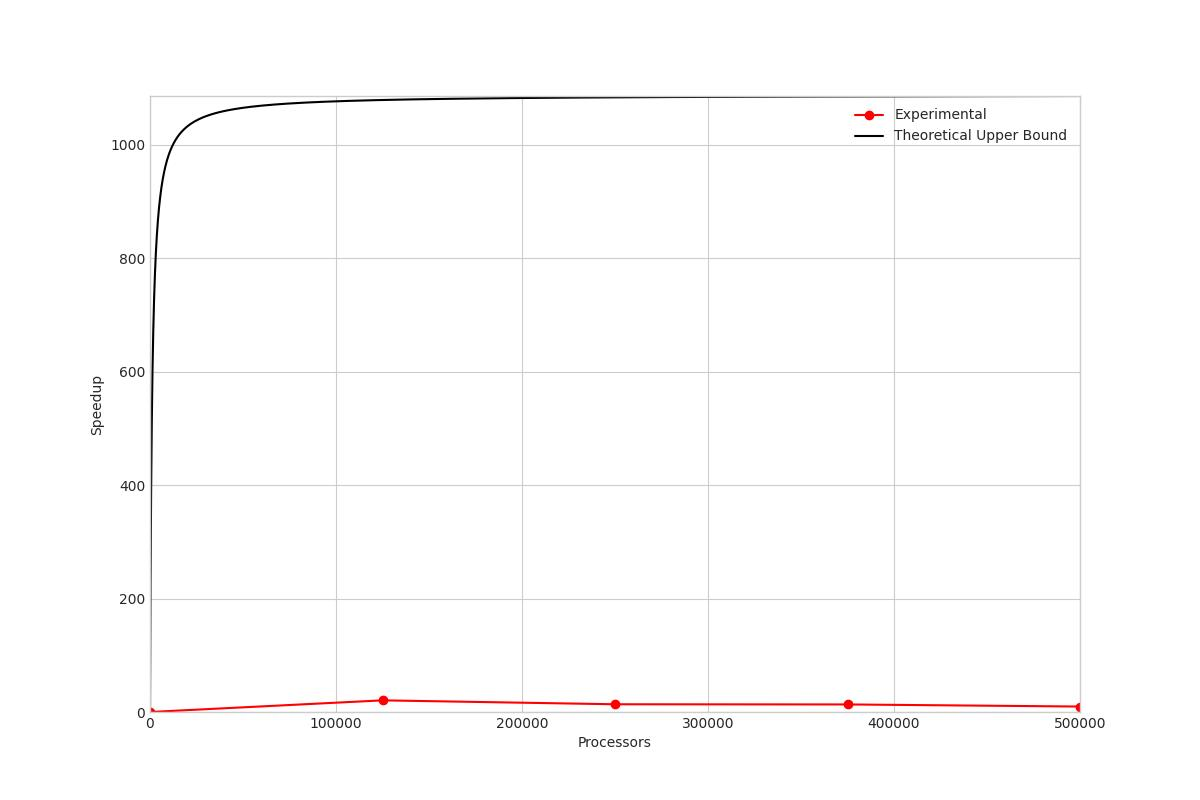
\includegraphics[width=0.74\textwidth]{../img/speedup-graph_type-random-500000-O0}
\end{center}

\subsubsection{Optimization 1}
\begin{center}
    \resizebox{0.8\textwidth}{!}{\subfile{../tables/psize-graph_type-random-500000-O1-table}}
    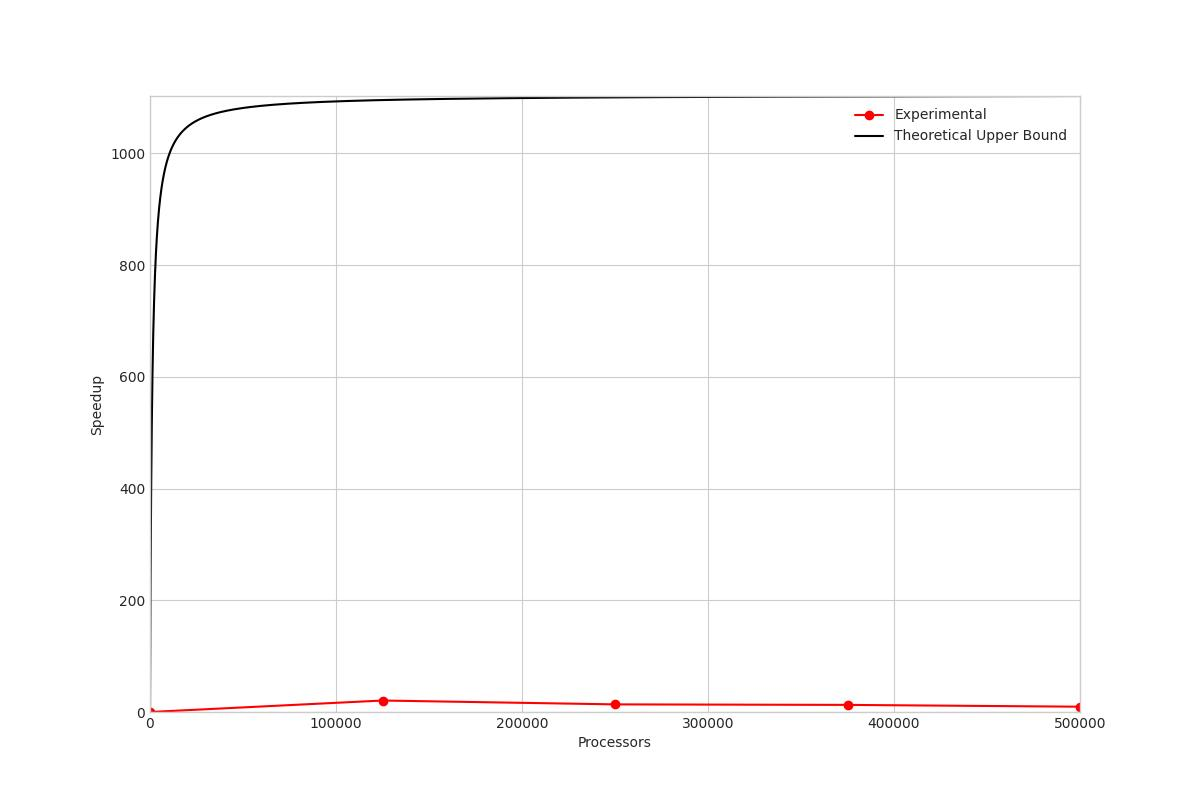
\includegraphics[width=0.74\textwidth]{../img/speedup-graph_type-random-500000-O1}
\end{center}

\clearpage
\subsubsection{Optimization 2}
\begin{center}
    \resizebox{0.8\textwidth}{!}{\subfile{../tables/psize-graph_type-random-500000-O2-table}}
    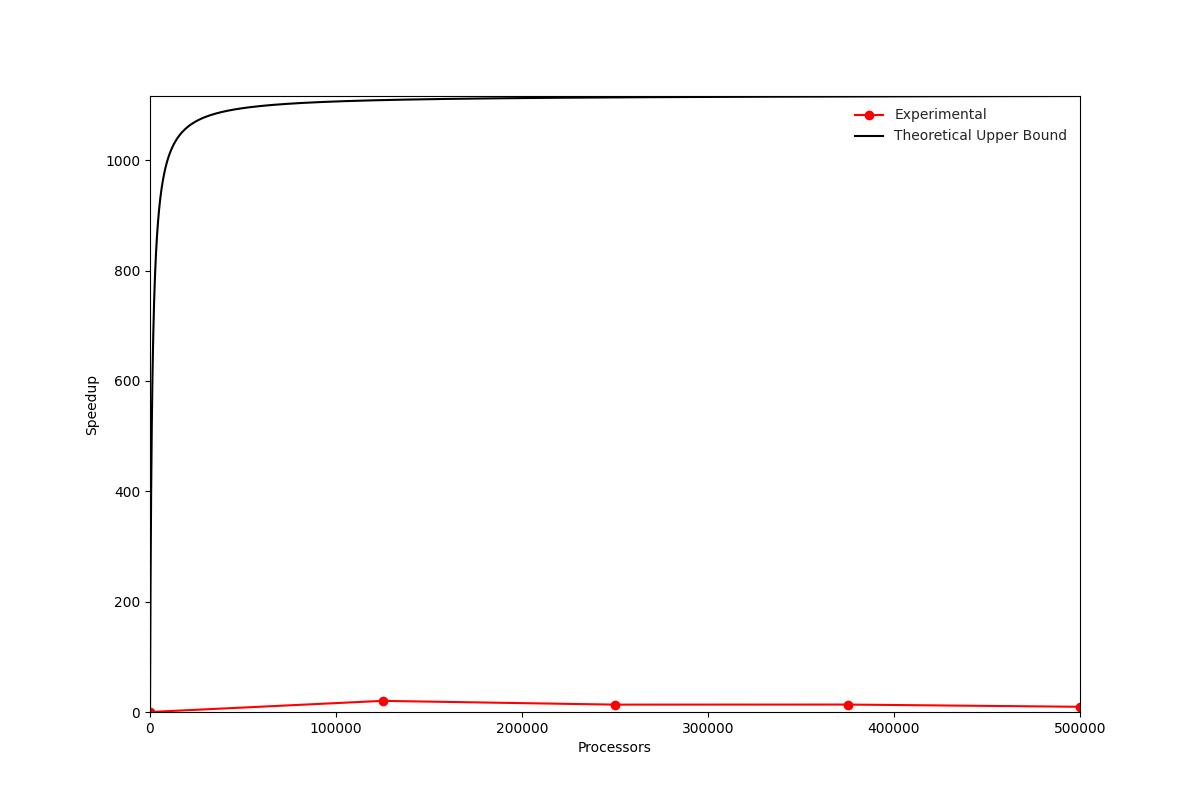
\includegraphics[width=0.78\textwidth]{../img/speedup-graph_type-random-500000-O2}
\end{center}

\subsubsection{Optimization 3}
\begin{center}
    \resizebox{0.8\textwidth}{!}{\subfile{../tables/psize-graph_type-random-500000-O3-table}}
    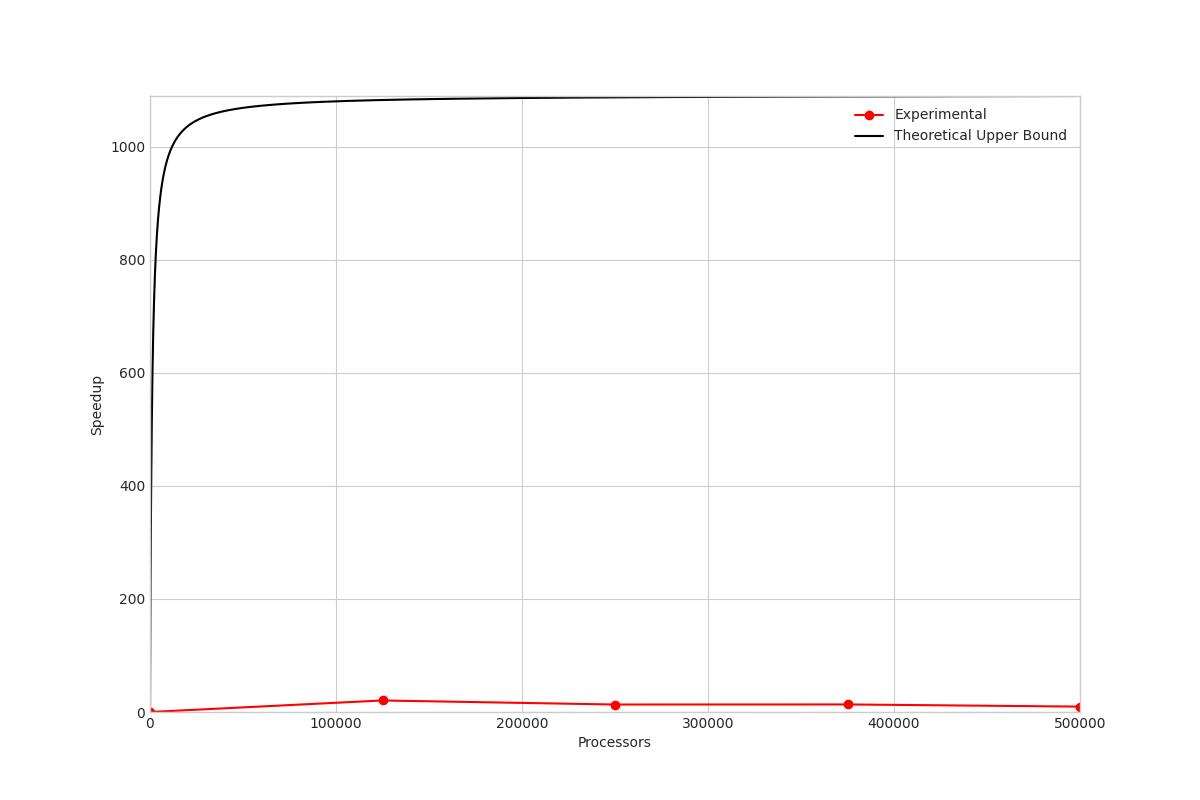
\includegraphics[width=0.78\textwidth]{../img/speedup-graph_type-random-500000-O3}
\end{center}

%Tile-52000 graph
\clearpage
\subsection{Tile-52000 graph}
\subsubsection{Optimization 0}
\begin{center}
    \resizebox{0.8\textwidth}{!}{\subfile{../tables/psize-graph_type-tile-52000-O0-table}}
    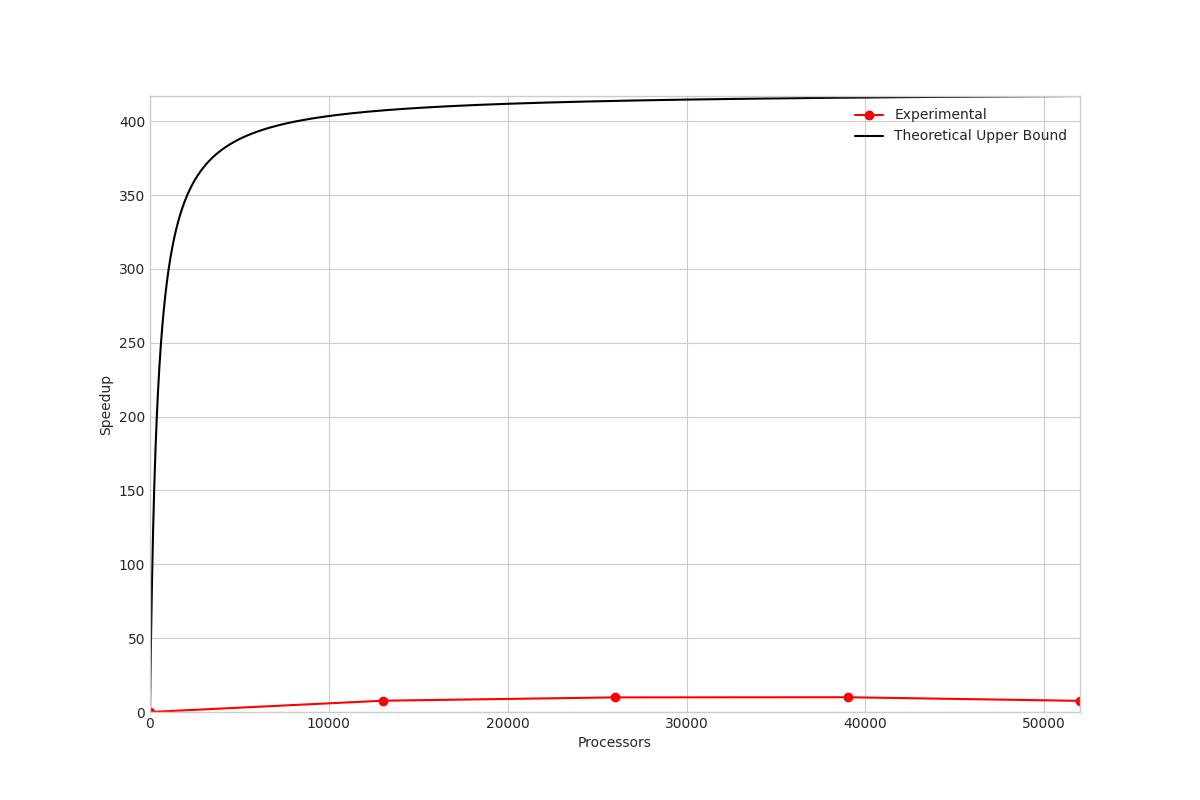
\includegraphics[width=0.73\textwidth]{../img/speedup-graph_type-tile-52000-O0}
\end{center}

\subsubsection{Optimization 1}
\begin{center}
    \resizebox{0.8\textwidth}{!}{\subfile{../tables/psize-graph_type-tile-52000-O1-table}}
    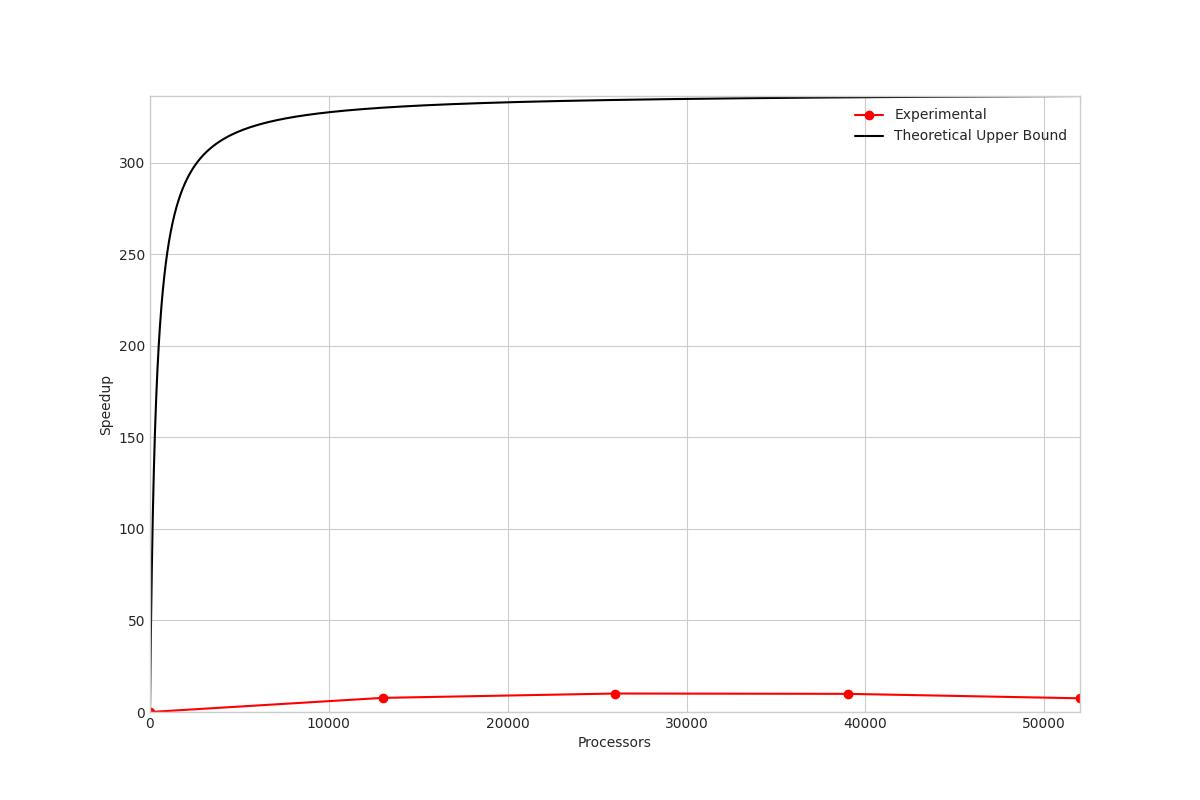
\includegraphics[width=0.74\textwidth]{../img/speedup-graph_type-tile-52000-O1}
\end{center}

\clearpage
\subsubsection{Optimization 2}
\begin{center}
    \resizebox{0.8\textwidth}{!}{\subfile{../tables/psize-graph_type-tile-52000-O2-table}}
    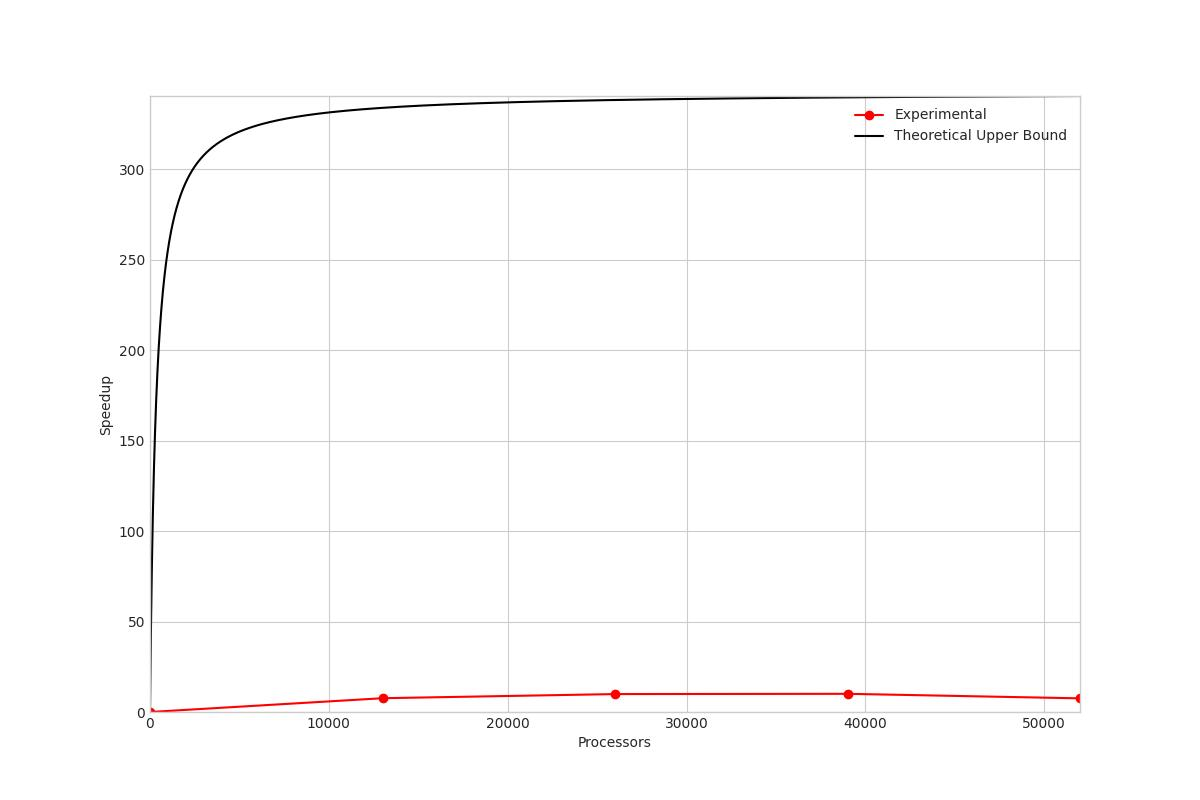
\includegraphics[width=0.77\textwidth]{../img/speedup-graph_type-tile-52000-O2}
\end{center}

\subsubsection{Optimization 3}
\begin{center}
    \resizebox{0.8\textwidth}{!}{\subfile{../tables/psize-graph_type-tile-52000-O3-table}}
    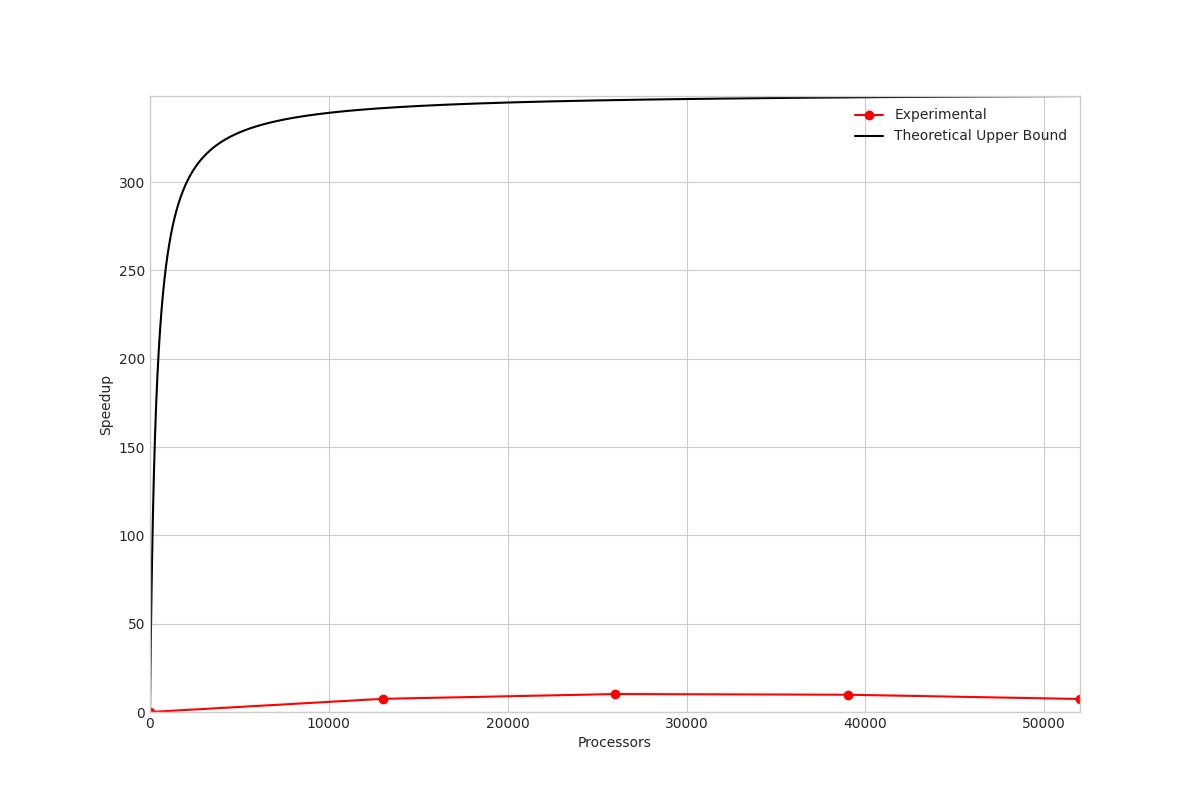
\includegraphics[width=0.77\textwidth]{../img/speedup-graph_type-tile-52000-O3}
\end{center}

%Tile-205000 graph
\clearpage
\subsection{Tile-205000 graph}
\subsubsection{Optimization 0}
\begin{center}
    \resizebox{0.8\textwidth}{!}{\subfile{../tables/psize-graph_type-tile-205000-O0-table}}
    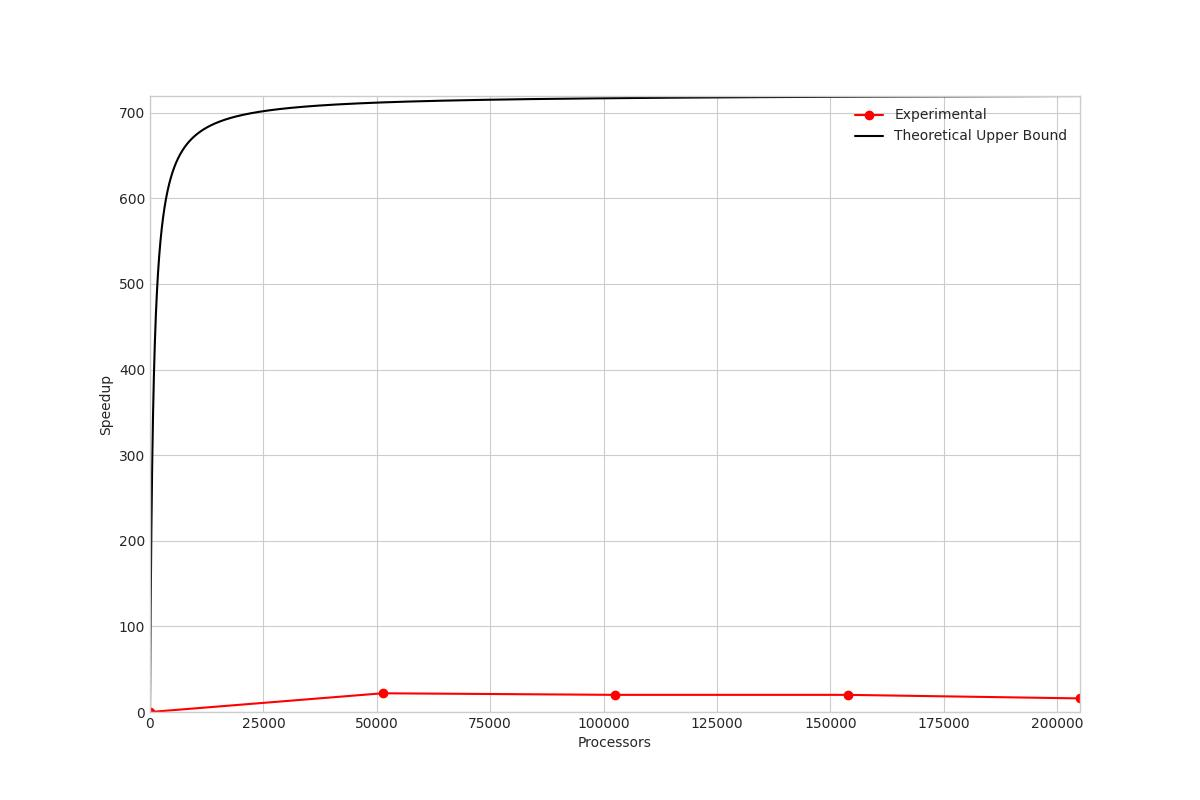
\includegraphics[width=0.74\textwidth]{../img/speedup-graph_type-tile-205000-O0}
\end{center}

\subsubsection{Optimization 1}
\begin{center}
    \resizebox{0.8\textwidth}{!}{\subfile{../tables/psize-graph_type-tile-205000-O1-table}}
    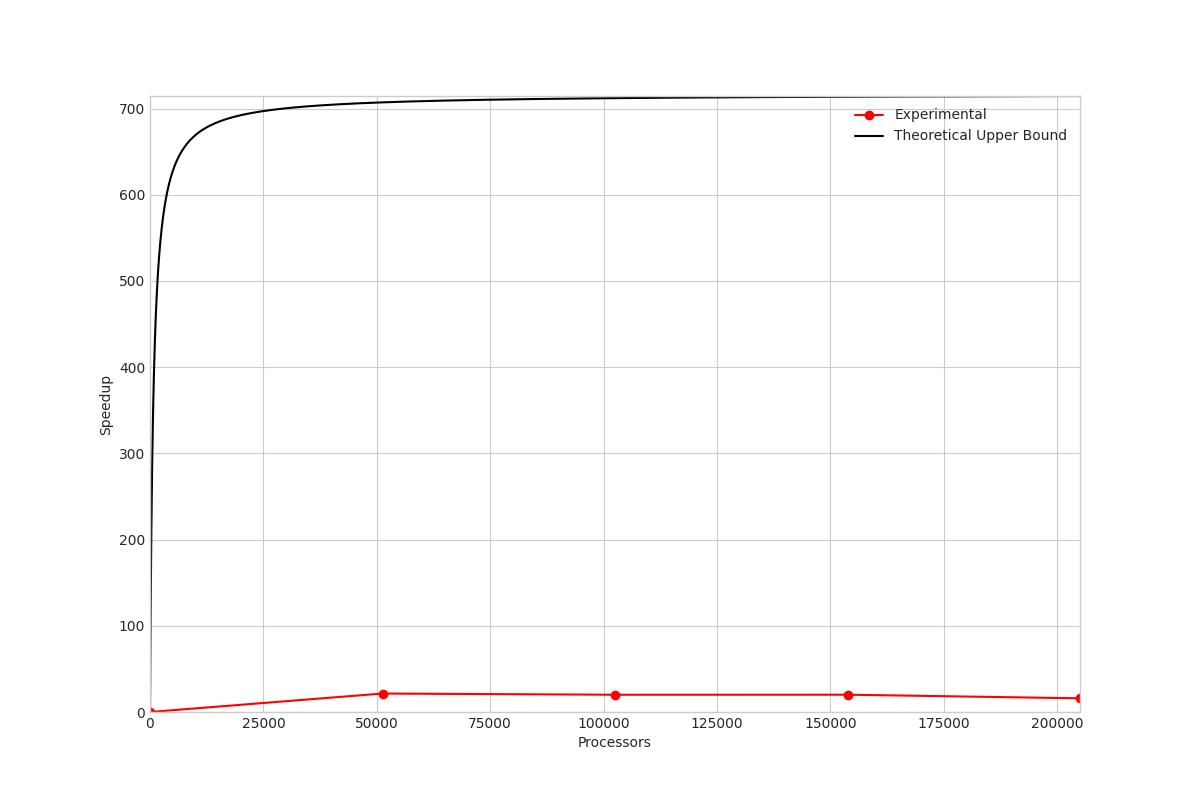
\includegraphics[width=0.74\textwidth]{../img/speedup-graph_type-tile-205000-O1}
\end{center}

\clearpage
\subsubsection{Optimization 2}
\begin{center}
    \resizebox{0.8\textwidth}{!}{\subfile{../tables/psize-graph_type-tile-205000-O2-table}}
    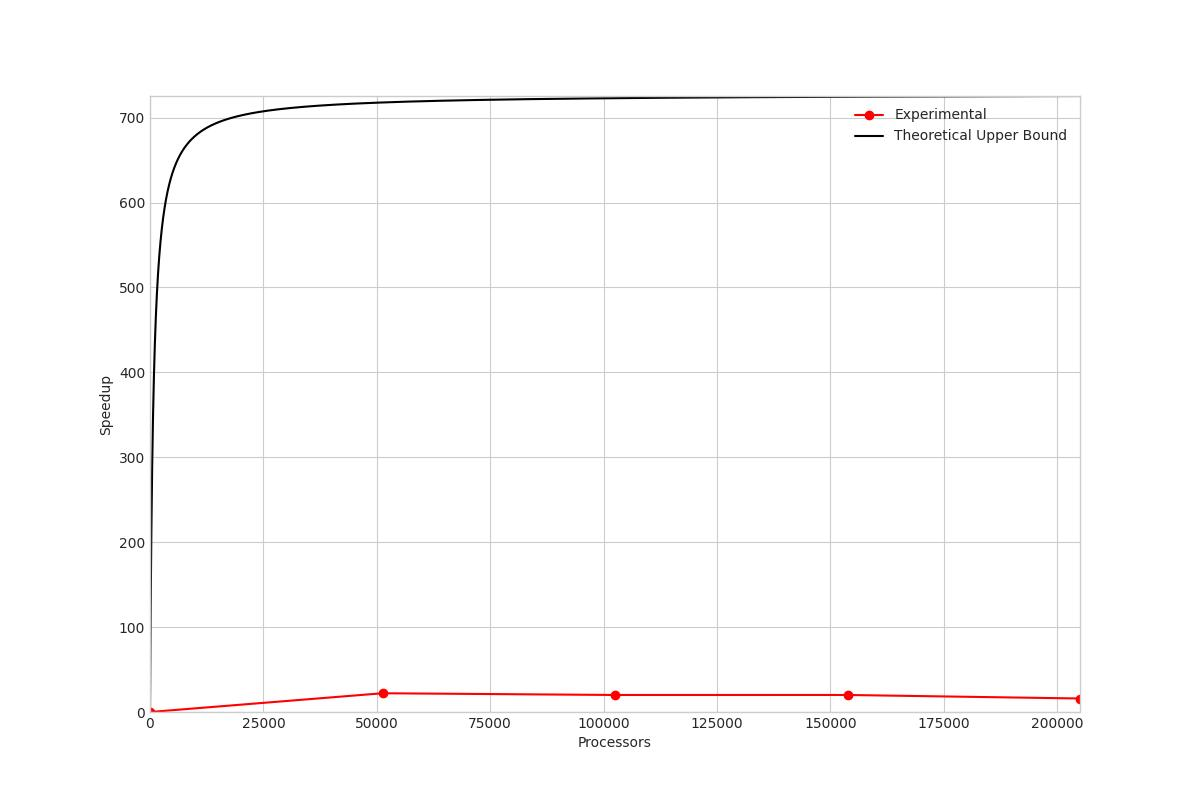
\includegraphics[width=0.78\textwidth]{../img/speedup-graph_type-tile-205000-O2}
\end{center}

\subsubsection{Optimization 3}
\begin{center}
    \resizebox{0.8\textwidth}{!}{\subfile{../tables/psize-graph_type-tile-205000-O3-table}}
    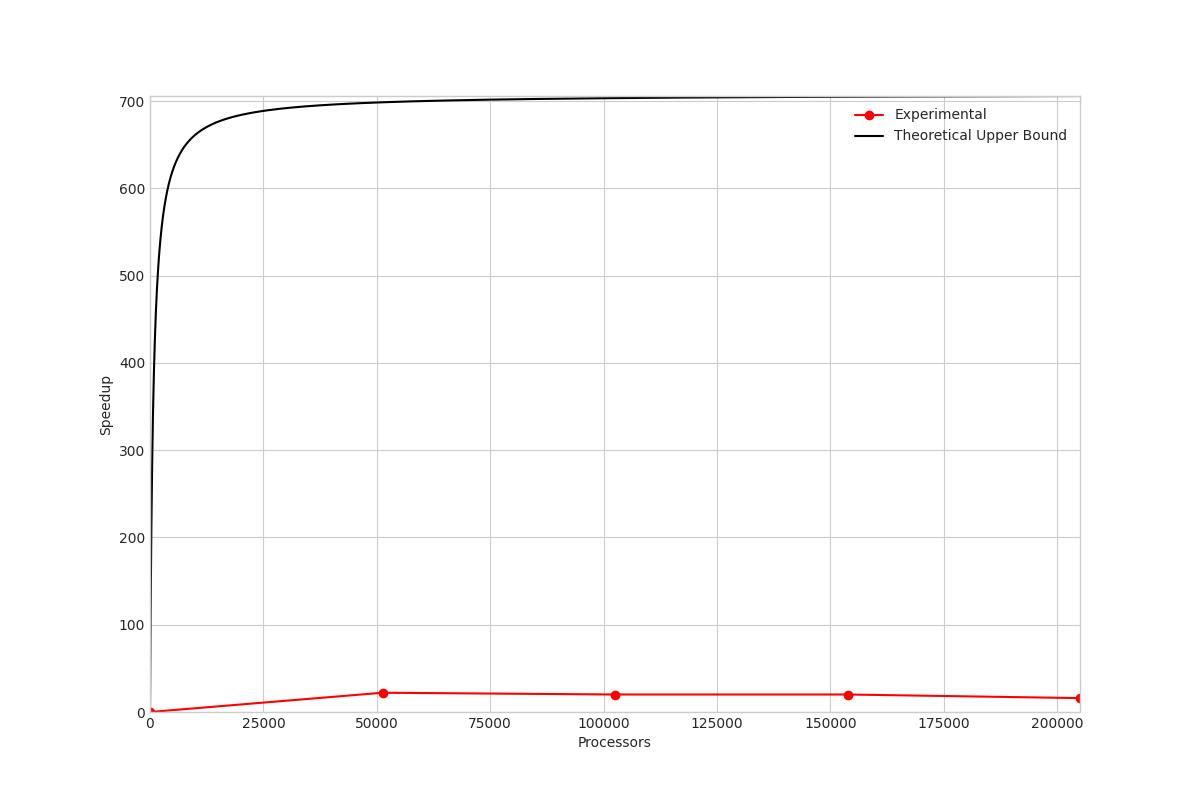
\includegraphics[width=0.78\textwidth]{../img/speedup-graph_type-tile-205000-O3}
\end{center}

%Tile-410000 graph
\clearpage
\subsection{Tile-410000 graph}
\subsubsection{Optimization 0}
\begin{center}
    \resizebox{0.8\textwidth}{!}{\subfile{../tables/psize-graph_type-tile-410000-O0-table}}
    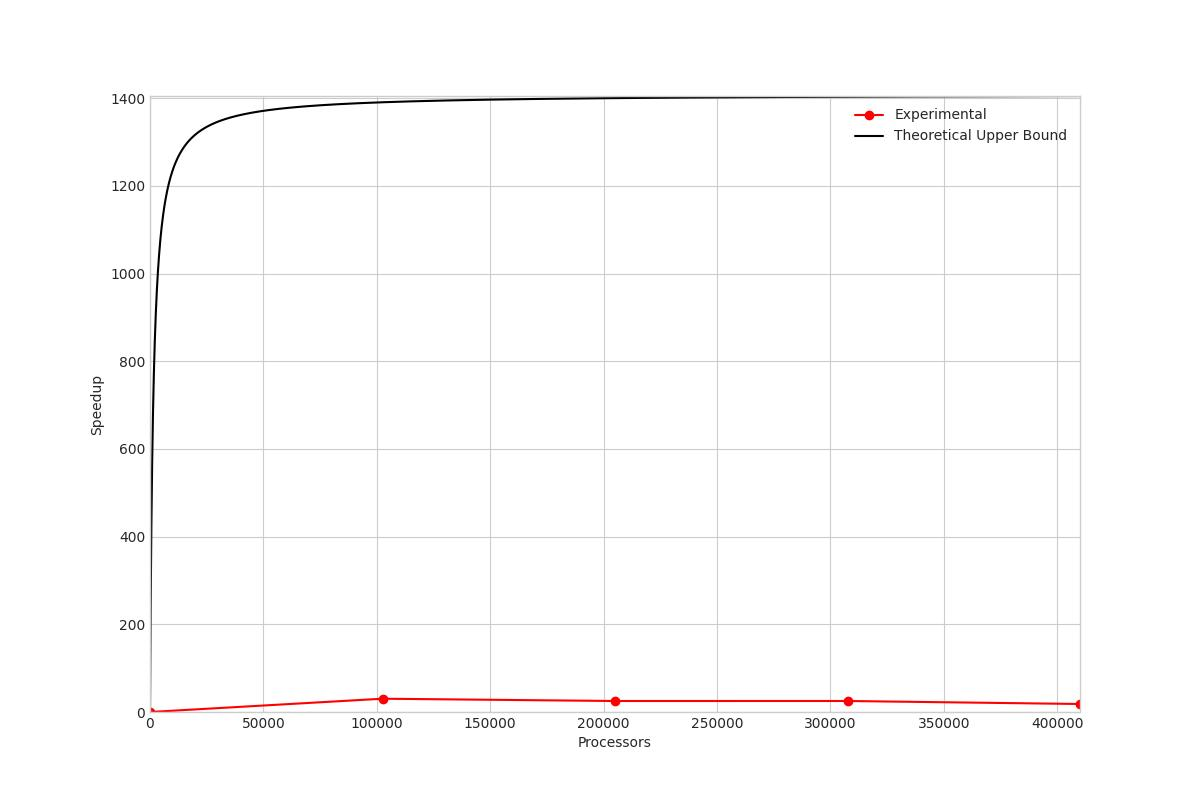
\includegraphics[width=0.74\textwidth]{../img/speedup-graph_type-tile-410000-O0}
\end{center}


\subsubsection{Optimization 1}
\begin{center}
    \resizebox{0.8\textwidth}{!}{\subfile{../tables/psize-graph_type-tile-410000-O1-table}}
    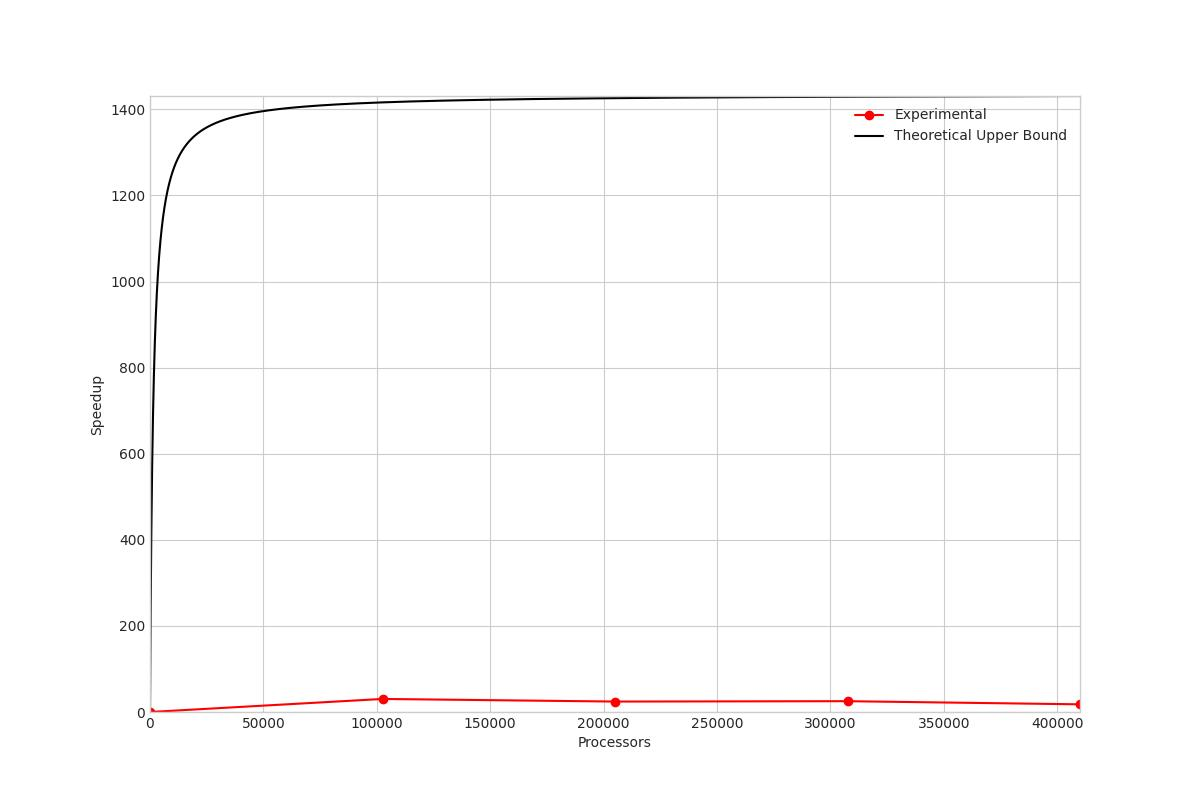
\includegraphics[width=0.74\textwidth]{../img/speedup-graph_type-tile-410000-O1}
\end{center}

\clearpage
\subsubsection{Optimization 2}
\begin{center}
    \resizebox{0.8\textwidth}{!}{\subfile{../tables/psize-graph_type-tile-410000-O2-table}}
    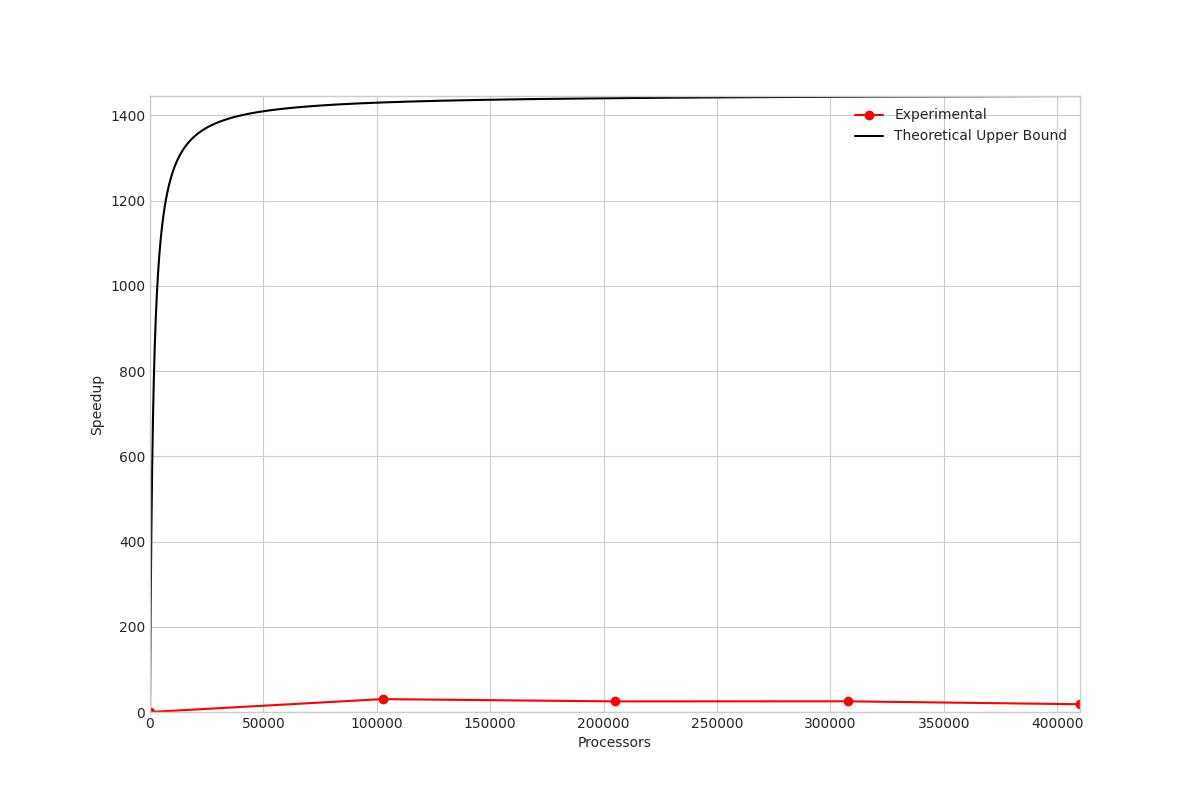
\includegraphics[width=0.78\textwidth]{../img/speedup-graph_type-tile-410000-O2}
\end{center}

\subsubsection{Optimization 3}
\begin{center}
    \resizebox{0.8\textwidth}{!}{\subfile{../tables/psize-graph_type-tile-410000-O3-table}}
    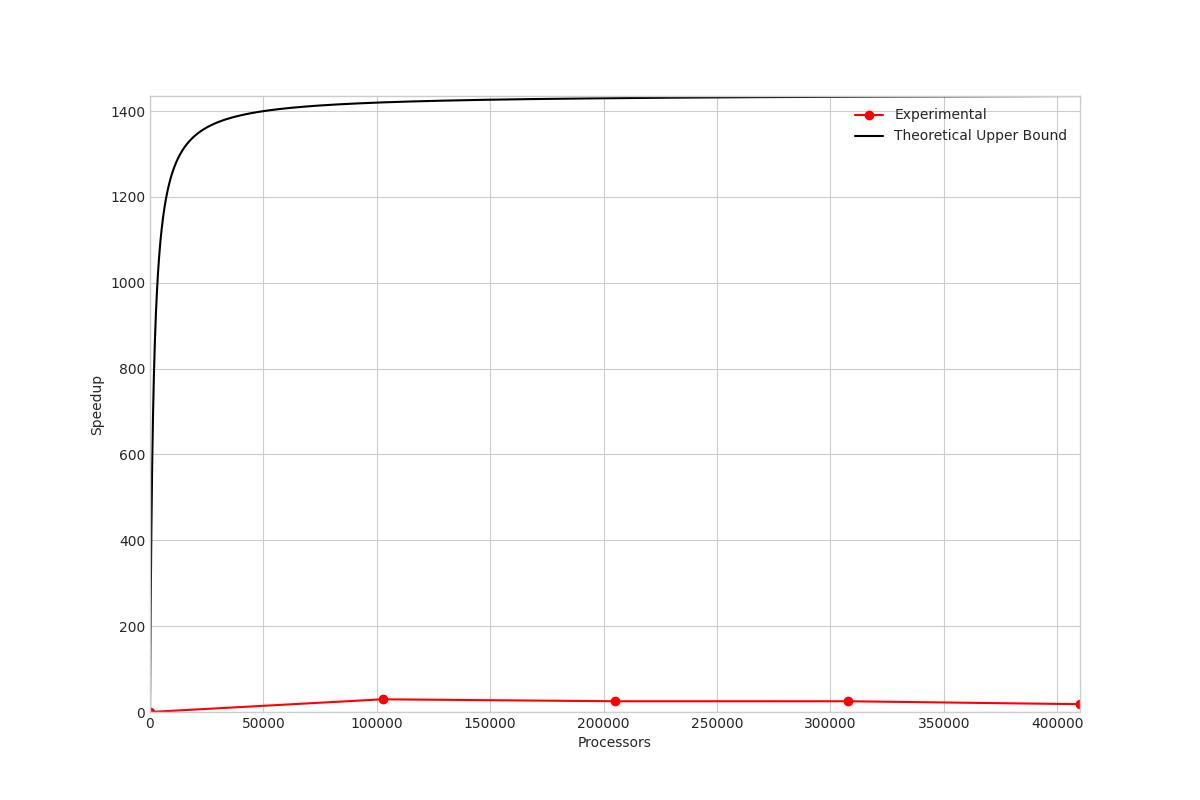
\includegraphics[width=0.78\textwidth]{../img/speedup-graph_type-tile-410000-O3}
\end{center}

%Tile-820000 graph
\clearpage
\subsection{Tile-820000 graph}
\subsubsection{Optimization 0}
\begin{center}
    \resizebox{0.8\textwidth}{!}{\subfile{../tables/psize-graph_type-tile-820000-O0-table}}
    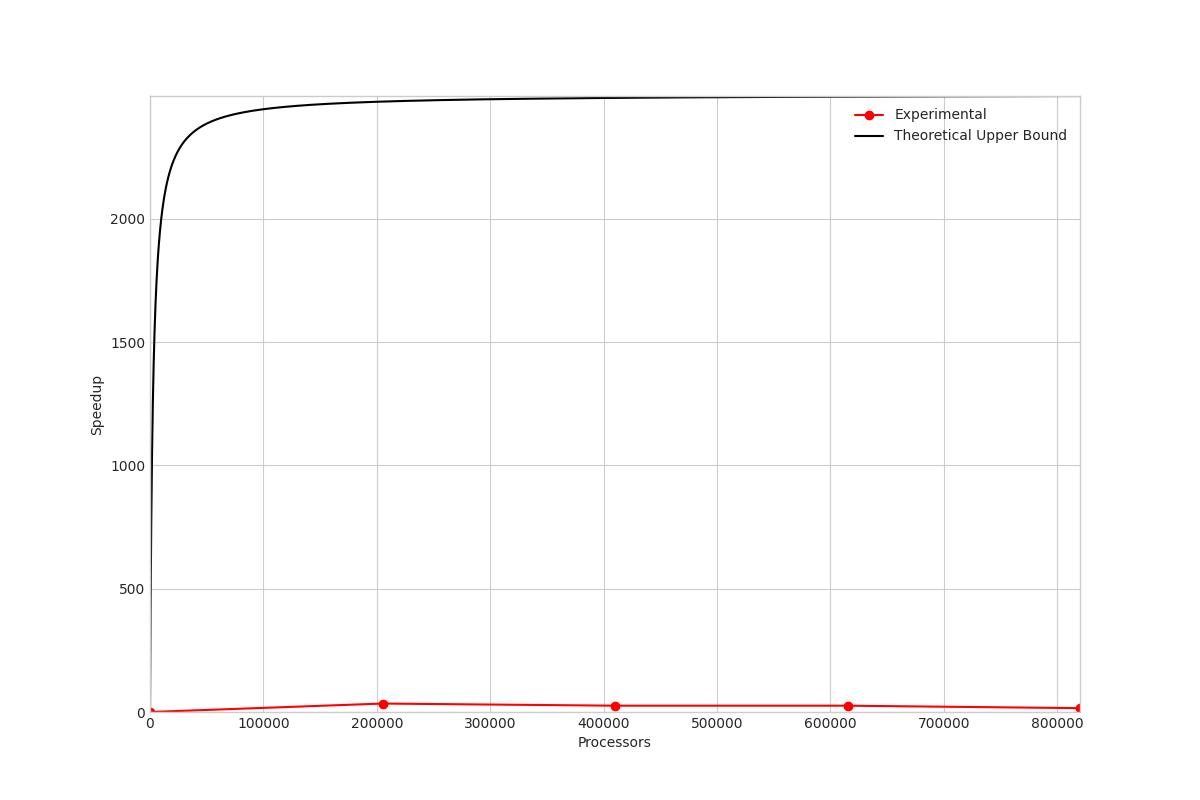
\includegraphics[width=0.74\textwidth]{../img/speedup-graph_type-tile-820000-O0}
\end{center}

\subsubsection{Optimization 1}
\begin{center}
    \resizebox{0.8\textwidth}{!}{\subfile{../tables/psize-graph_type-tile-820000-O1-table}}
    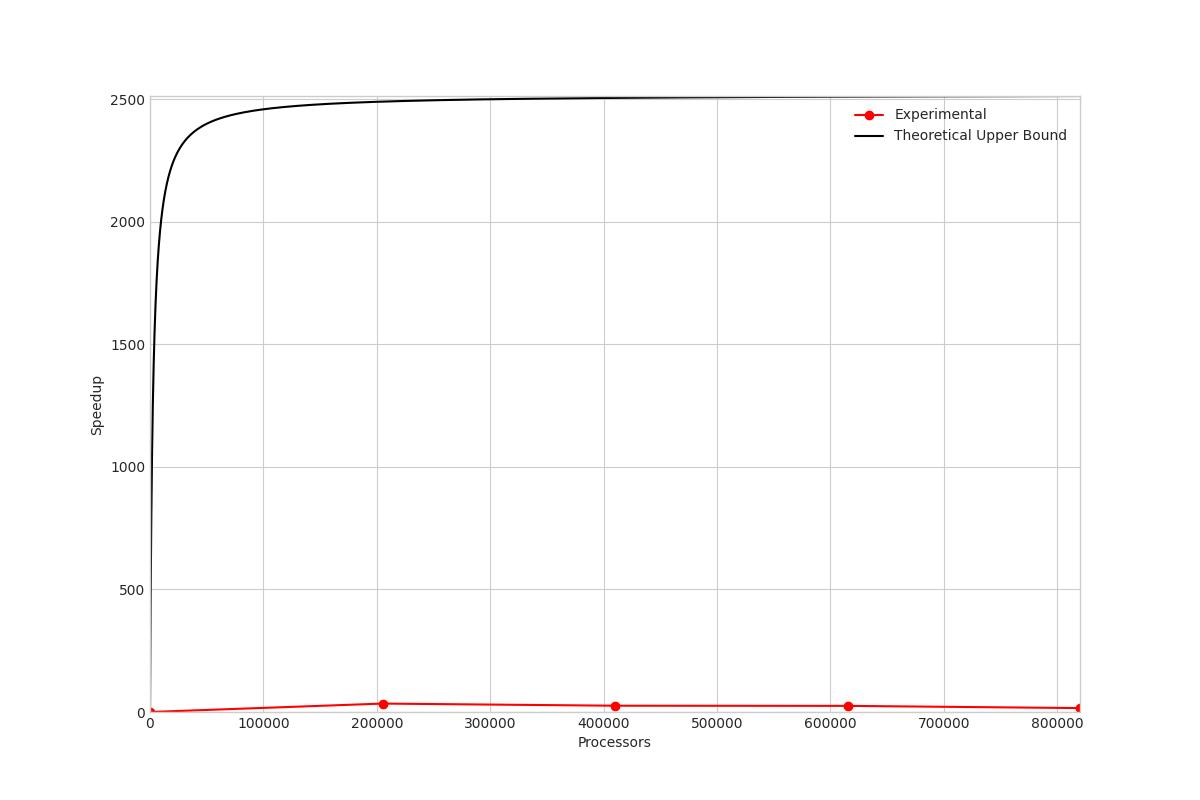
\includegraphics[width=0.74\textwidth]{../img/speedup-graph_type-tile-820000-O1}
\end{center}

\clearpage
\subsubsection{Optimization 2}
\begin{center}
    \resizebox{0.8\textwidth}{!}{\subfile{../tables/psize-graph_type-tile-820000-O2-table}}
    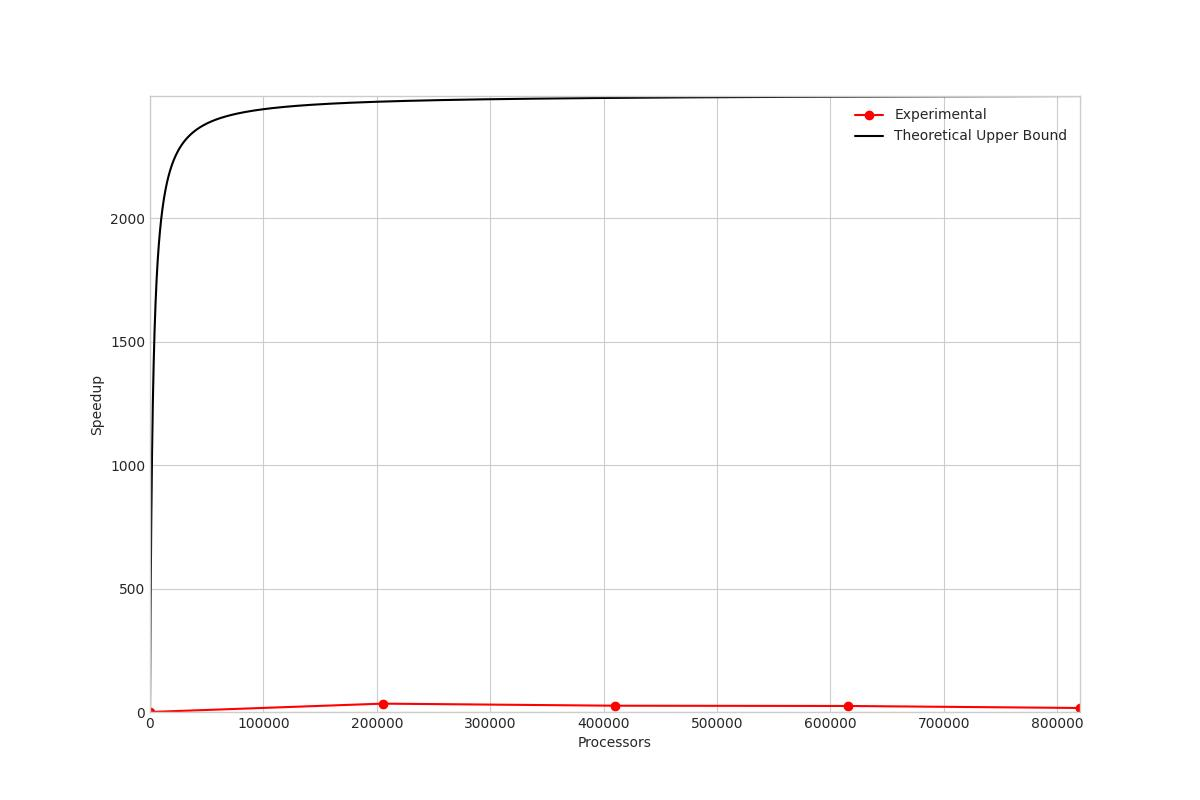
\includegraphics[width=0.78\textwidth]{../img/speedup-graph_type-tile-820000-O2}
\end{center}

\subsubsection{Optimization 3}
\begin{center}
    \resizebox{0.8\textwidth}{!}{\subfile{../tables/psize-graph_type-tile-820000-O3-table}}
    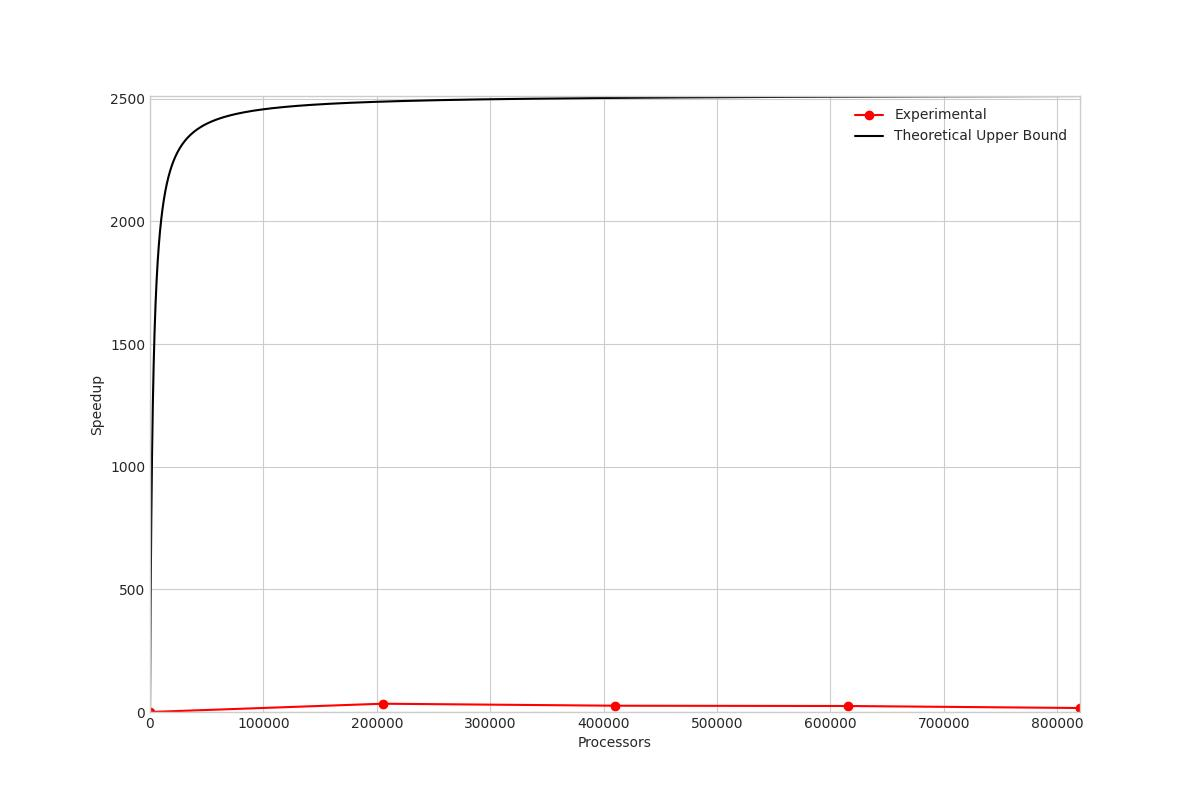
\includegraphics[width=0.78\textwidth]{../img/speedup-graph_type-tile-820000-O3}
\end{center}
